\section{Results}

In the previous section we defined a regime based trading strategy that uses an HMM as a times series forecasting model, which feeds into a model predictive control (MPC) framework to determine trading decisions. In this section results of the MPC strategy is evaluated and compared to a number of alternative portfolios. The analysis is divided between in-sample training and out-of-sample testing. The purpose of the in-sample training is to compute optimal values for hyperparameters of the forecast horizon and other hyperparameters in the MPC problem in \cref{eq: maximizing objective MPC}, while in the out-of-sample section, the MPC approach is evaluated using optimal parameters and compared to benchmarks. In the remainder of the section, we first present the data in- and out-of-sample, before describing the in-sample training after which out-of-sample results are presented.

\subsection{Data}

The full dataset covers the period form February 1994 to February 2021. Though some indices go further back, the choice of time period is a trade-off between historical availability and the size of the asset universe, with the latter significantly shrinking before 1994. The in-sample data, shown in \cref{fig:MPC_data_is}, runs from February 1994 to November 2003, resulting in 2539 daily observations. It covers the S\&P 500, MSCI Emerging Markets, Barclays US Treasury, CSI Barc Index, Gold and Oil\footnote{
The 6 indices are \textbf{Insert formal name of all indices as indice 1, indice 2 etc.}.
}.
Three month treasury bills are used as a benchmark for the risk-free asset. In the initial months where only monthly data is available for the risk-free asset, daily prices are linearly interpolated with some gaussian noise. We note that the first 1700 observations are used for initialization after which training commences. As this is a rather large slice of the in-sample data implications of this is discussed in greater detail in the coming sections. Finally, we note that the assets considered in-sample is only a subset of the assets considered out-of-sample due to data limitations. \textbf{Consider implications of this on the optimal MPC hyperparameters.}

\begin{figure}[H]
    \centering
    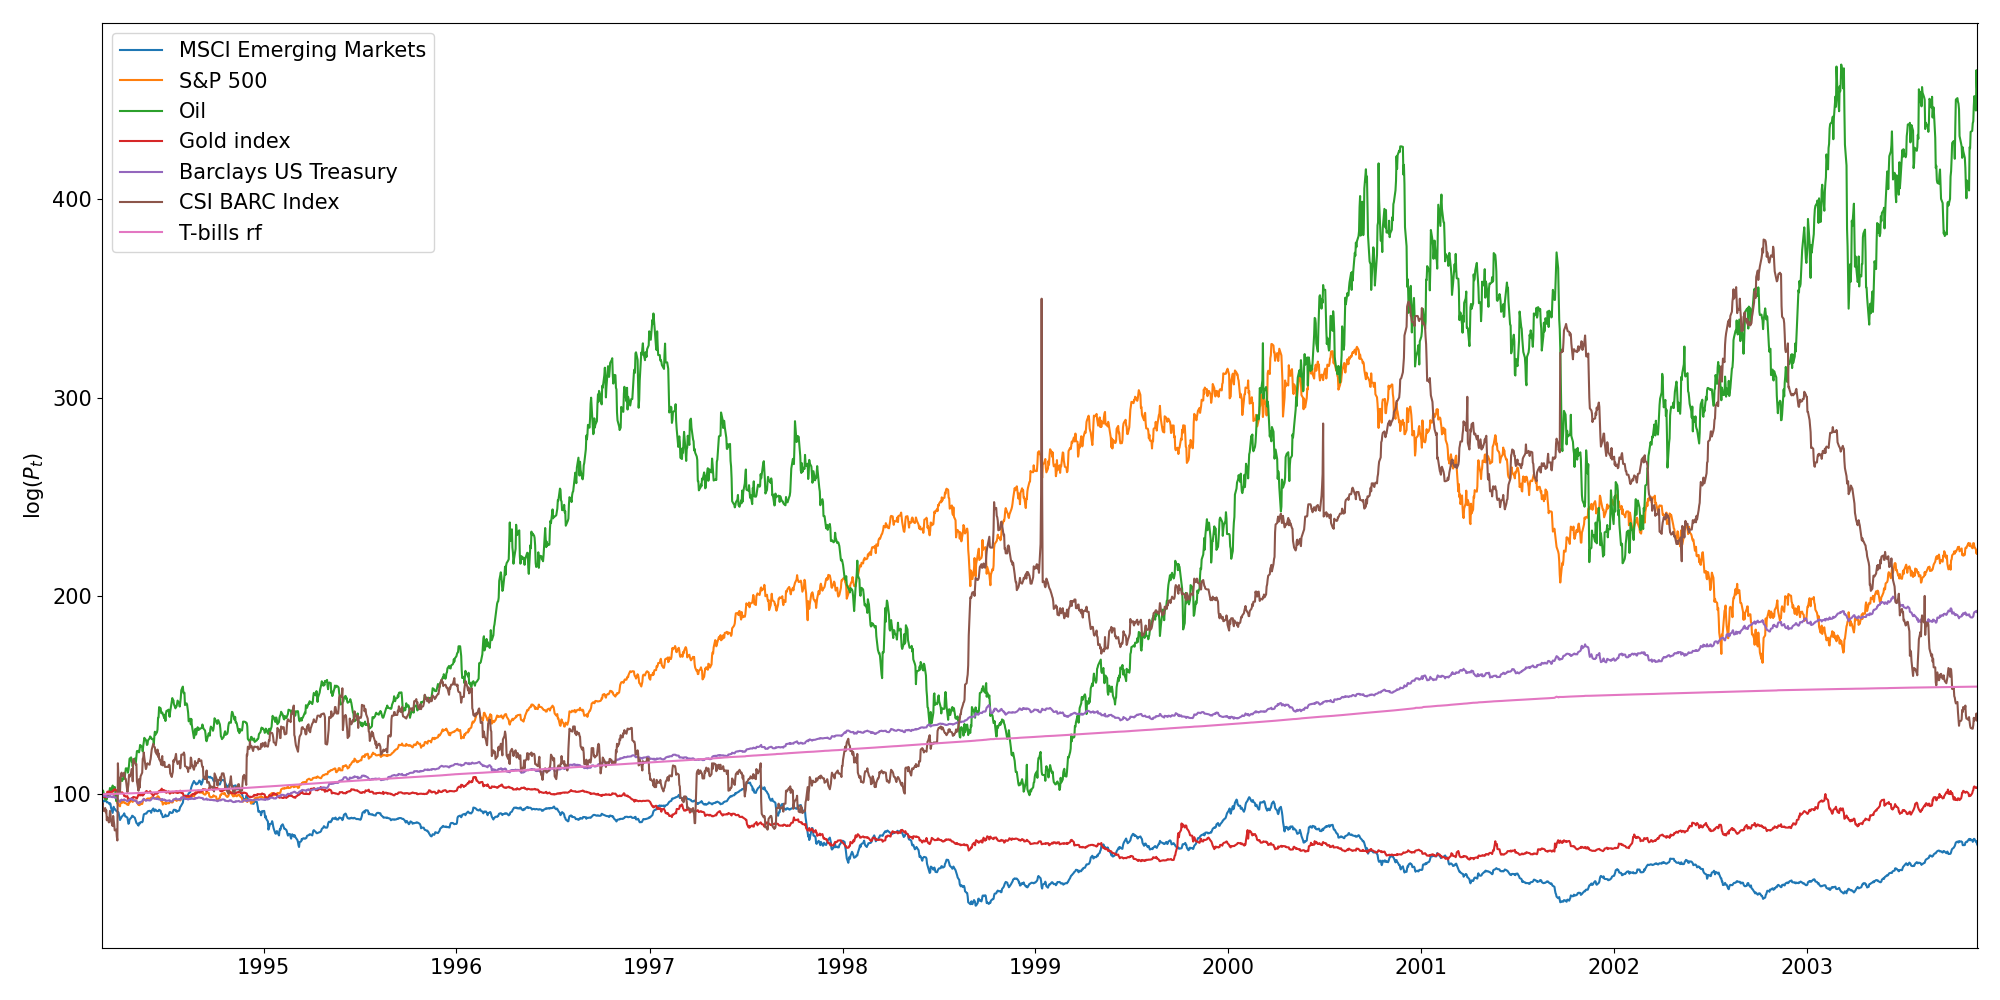
\includegraphics[width=1\textwidth]{analysis/portfolio_exercise/images/asset_vals_insample.png}
    \caption[Historical asset prices during the in-sample period]{Historical asset prices during the in-sample period.}
    \label{fig:MPC_data_is}
\end{figure}

The out-of-sample period runs from November 2003 to February 2021 resulting in 4495 daily observations. It is shown in \cref{fig:MPC_data_oos} It covers S\&P 500, MSCI Emerging Markets, Hedge Funds Global, Private Equity, European Public Real Estate, Gold, Oil, Barclays US Treasury and CSI Barc Index\footnote{
The 9 indices are \textbf{Insert formal name of all indices as indice 1, indice 2 etc.}.
}.
Again, the first years are used for initialization, meaning the the trading strategy is not implemented until September 2007, just before the financial crisis. This makes it an interesting period to study, as most assets had significant drawdowns during the crisis, and because it additionally includes the sovereign debt crisis in 2012 and the Covid-19 outbreak in 2020. As note by (\textbf{Insert REF}), asset correlations tend to increase during recessions, as can be seen in \cref{fig:MPC_data_oos}, meaning that many portfolios, such as an equally weighted or value weighted portfolio generally would suffer significant drawdowns in such periods. 

\begin{figure}[H]
    \centering
    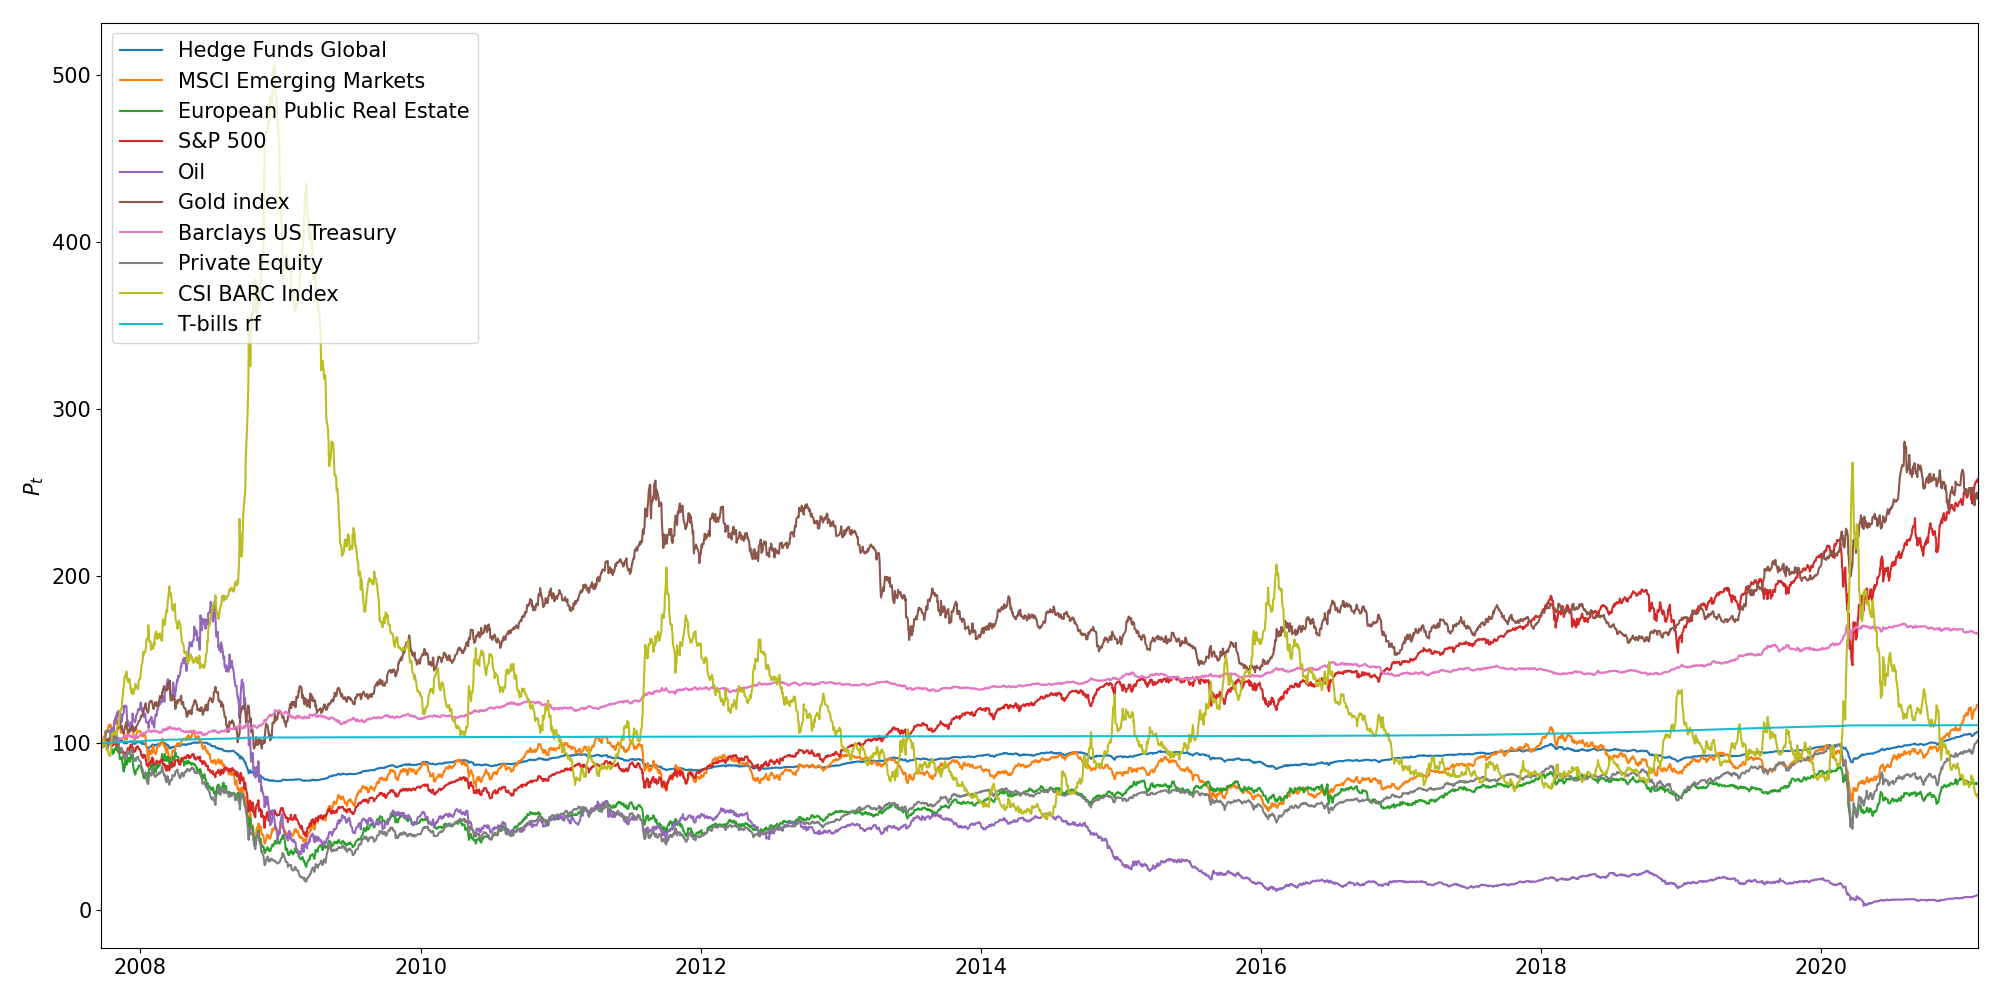
\includegraphics[width=1\textwidth]{analysis/portfolio_exercise/images/asset_vals_oos.png}
    \caption[Historical asset prices during the out-of-sample period]{Historical asset prices during the out-of-sample period. \textbf{Vis den fulde oos periode og forklar at de første 1700 observationer er brugt til initialization}}
    \label{fig:MPC_data_oos}
\end{figure}

Finally, \cref{tab:MPC_asset_performance} shows the annualized\footnote
{Daily returns are analyzed using
\begin{flalign*}
    \mu_{annual} &= (1+\mu_{daily})^{1/252}-1 \\
    \Sigma_{annual} &= {\Sigma}_{daily} * 252
\end{flalign*}
}
asset performance. 

\begin{table}[H]
\centering
\caption[Annualized
performance for each asset during the out-of-sample period]{Annualized
performance for each asset during the out-of-sample period. All measures are in excess of the risk-free rate.}
\begin{tabular}{lrrrrrrr}
\toprule
{} &  return &     std &  excess\_return &  excess\_std &  sharpe &  max\_drawdown &  calmar\_ratio \\
\midrule
MSCI World            &  0.0338 &  0.1638 &         0.0180 &      0.1641 &  0.1094 &        0.5907 &        0.0304 \\
MSCI Emerging Markets &  0.0591 &  0.1869 &         0.0429 &      0.1872 &  0.2291 &        0.6606 &        0.0649 \\
S\&P 500               &  0.0459 &  0.1923 &         0.0299 &      0.1925 &  0.1553 &        0.5678 &        0.0527 \\
Oil                   & -0.0800 &  0.3928 &        -0.0941 &      0.3929 & -0.2395 &        0.9852 &       -0.0955 \\
Gold index            &  0.0929 &  0.1681 &         0.0762 &      0.1680 &  0.4537 &        0.4462 &        0.1708 \\
Barclays US Treasury  &  0.0427 &  0.0443 &         0.0268 &      0.0440 &  0.6099 &        0.0717 &        0.3742 \\
CSI BARC Index        & -0.0428 &  0.3155 &        -0.0573 &      0.3153 & -0.1818 &        0.8925 &       -0.0642 \\
port\_val              &  0.0530 &  0.0967 &         0.0370 &      0.0965 &  0.3828 &        0.2671 &        0.1384 \\
\bottomrule
\end{tabular}

\label{tab:MPC_asset_performance}
\end{table}


\subsection{In-sample training: Tuning hyperparameters}

\textbf{We test the MPC model in sampler over the following grid: Forecasts period $H=1, 10,15,25$, transaction costs $\kappa_1= 0.0005, 0.001, 0.004, 0.008, 0.012, 0.015$, holding costs $\rho_2=0, 0.0005, 0.001, 0.002$ and a maximum holding constraint $w_{max}=0.2, 0.3, 0.4, 0.5$. This results in $4\cdot6\cdot4\cdot4=384$ different combinations. Doing the full gridsearch takes roughly 48 hours on a single core. All training is carried out for a long-only portfolio with $\gamma_0=5$ because that results in excess risk similar to the 1/n portfolio.}

\textbf{In choosing the optimal parameters, we consider the three objectives max Sharpe ratio, max Calmar ratio and min Annual portfolio turnover. Optimal values are found as H=15, transaction costs $\kappa_1$=0.0010, holding costs $\rho_2=0$, and a maxmimum holding constraint of $w_{max}=0.2$.}

\begin{itemize}
    \item Sample period
    \item method - what do we maximize
    \item go over each tuning parameter separately.
\end{itemize}


\subsection{Out-of-sample results}


\subsubsection*{Allocations}

\textbf{A very large allocation is in the risky asset across most time periods. This is likely due to it having a very low covariance with other assets and thus being desirable in a mean-variance setting - is there some clever way to reduce the overall allocation to rf?}

\textbf{Consider adding allocation plots with and without drawdown control to see difference. Currently showing with drawdown control}

\begin{figure}[H]
    \centering
    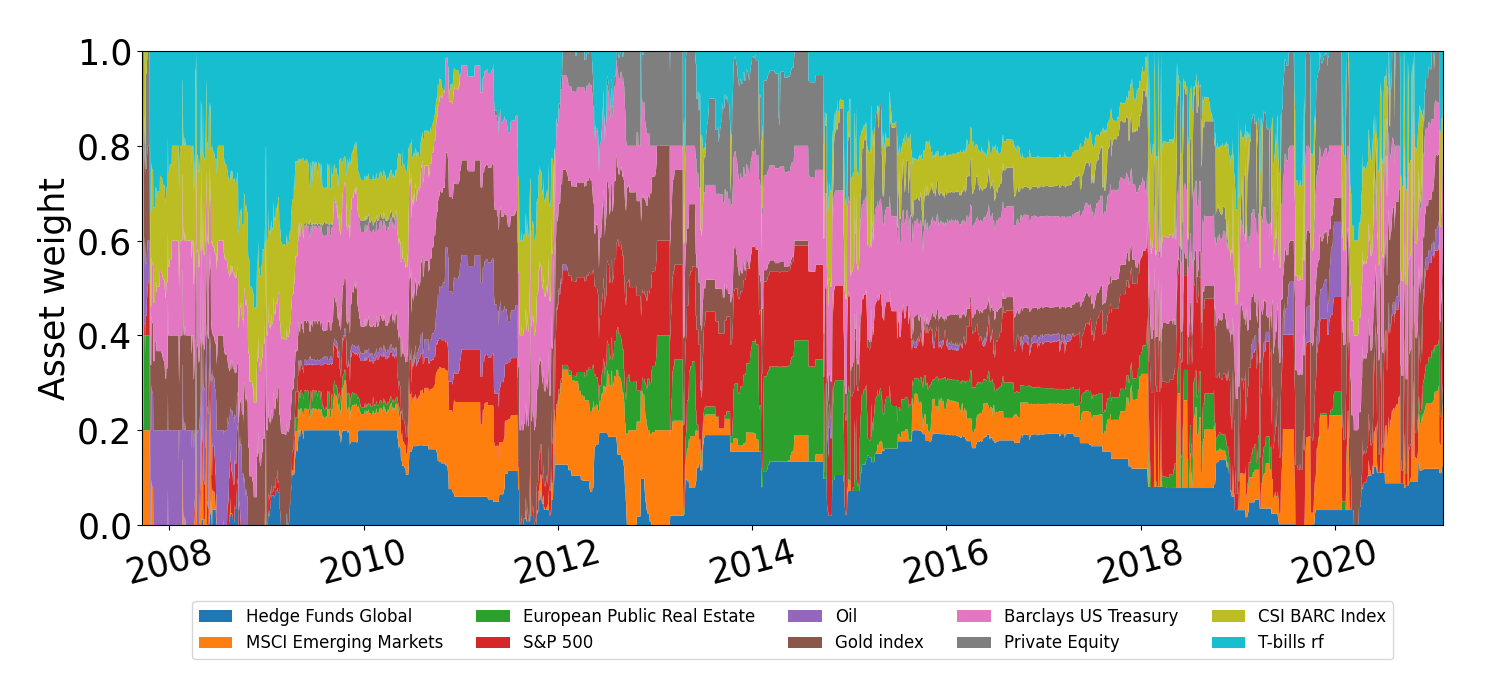
\includegraphics[width=1\textwidth]{analysis/portfolio_exercise/images/mle/weights_lo.png}
    \caption[Asset weights over time for a long-only portfolio]{Asset weights over time for a long-only portfolio.}
    \label{fig:MPC_port_weights_lo}
\end{figure}

\begin{figure}[H]
    \centering
    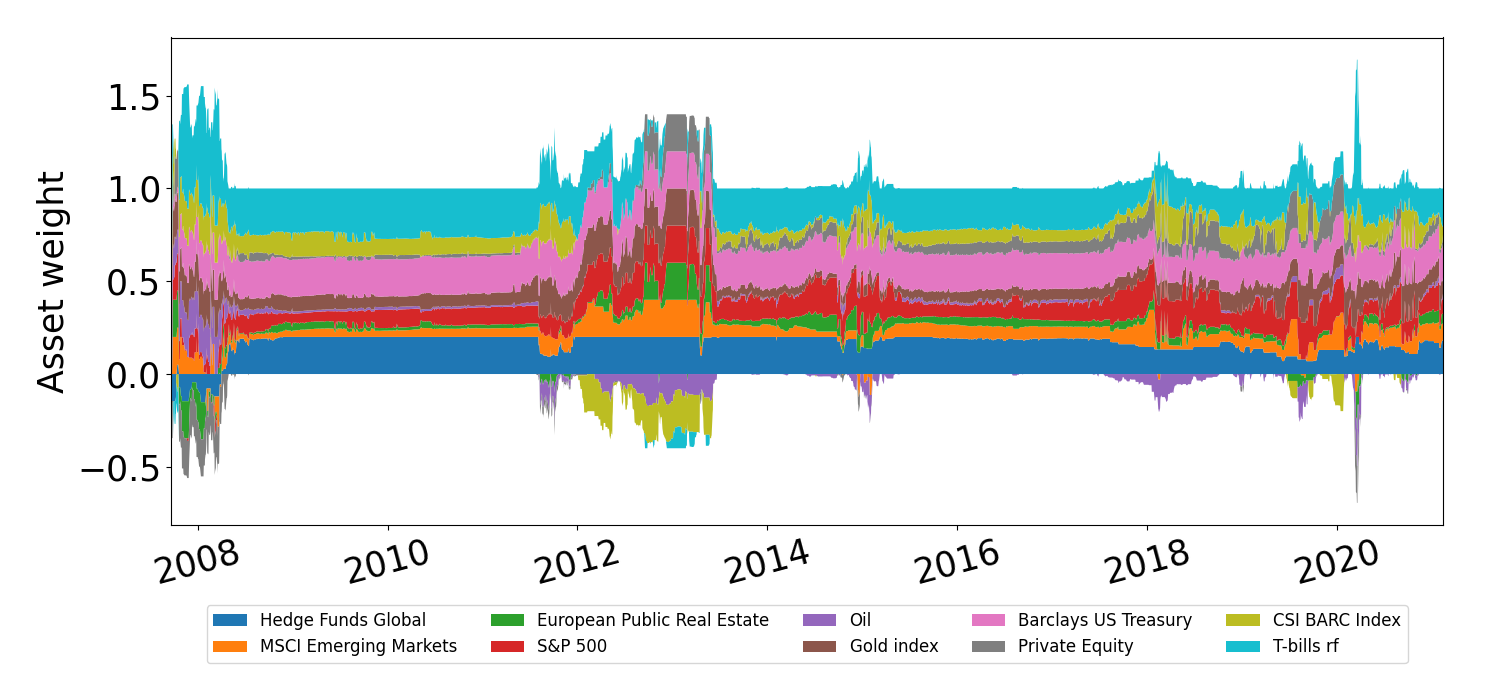
\includegraphics[width=1\textwidth]{analysis/portfolio_exercise/images/mle/weights_ls.png}
    \caption[Asset weights over time for a long-short portfolio]{Asset weights over time for a long-short portfolio.}
    \label{fig:MPC_port_weights_ls}
\end{figure}

\begin{figure}[H]
    \centering
    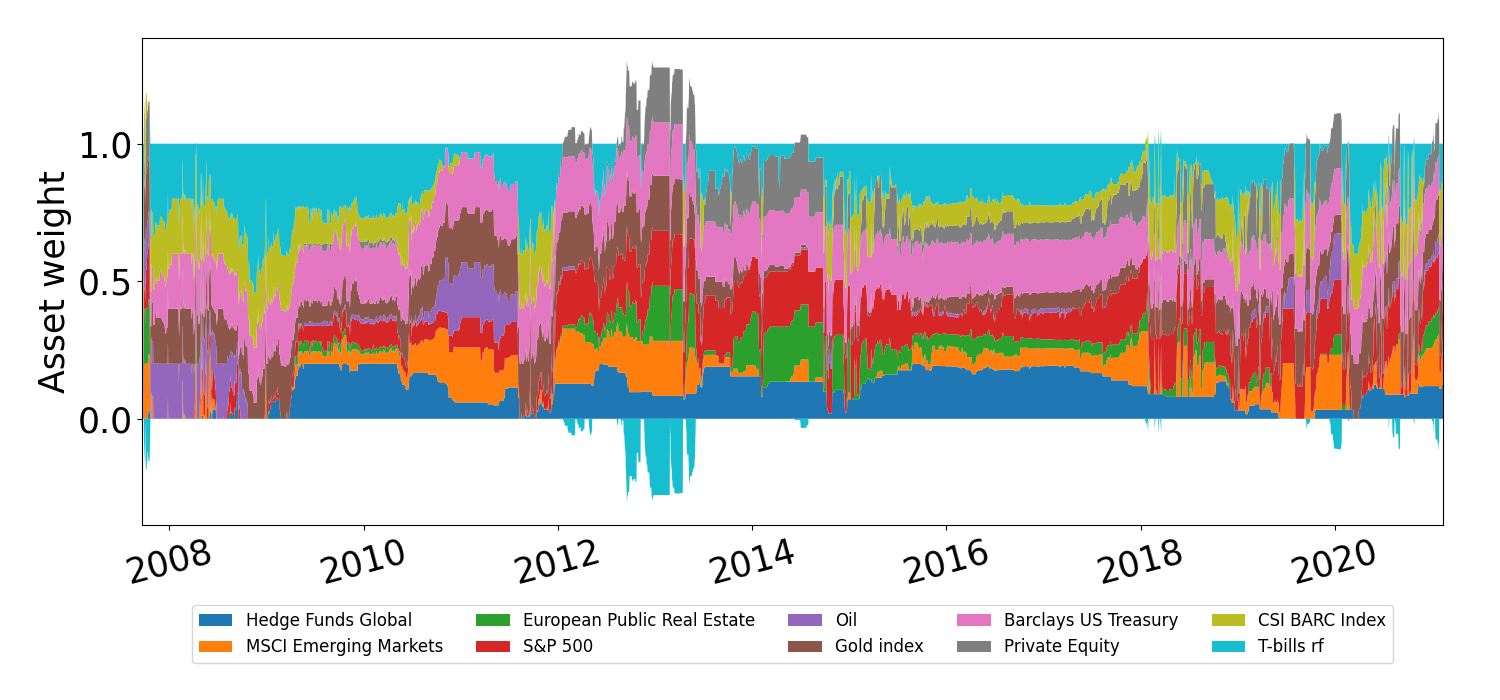
\includegraphics[width=1\textwidth]{analysis/portfolio_exercise/images/mle/weights_llo.png}
    \caption[Asset weights over time for a leveraged long-only portfolio]{Asset weights over time for a leveraged long-only portfolio.}
    \label{fig:MPC_port_weights_llo}
\end{figure}

\subsubsection*{Performance comparison}

\textbf{$D_{max}$ indikerer den maksimale drawdown tolerance. Hvis en portefølje når $D_{max}$, går risikoaversionen $\gamma$ mod uendelig. Alle plots er efter transaction costs på 10 basispoint per one-way transaktion.}

\begin{figure}[H]
    \centering
    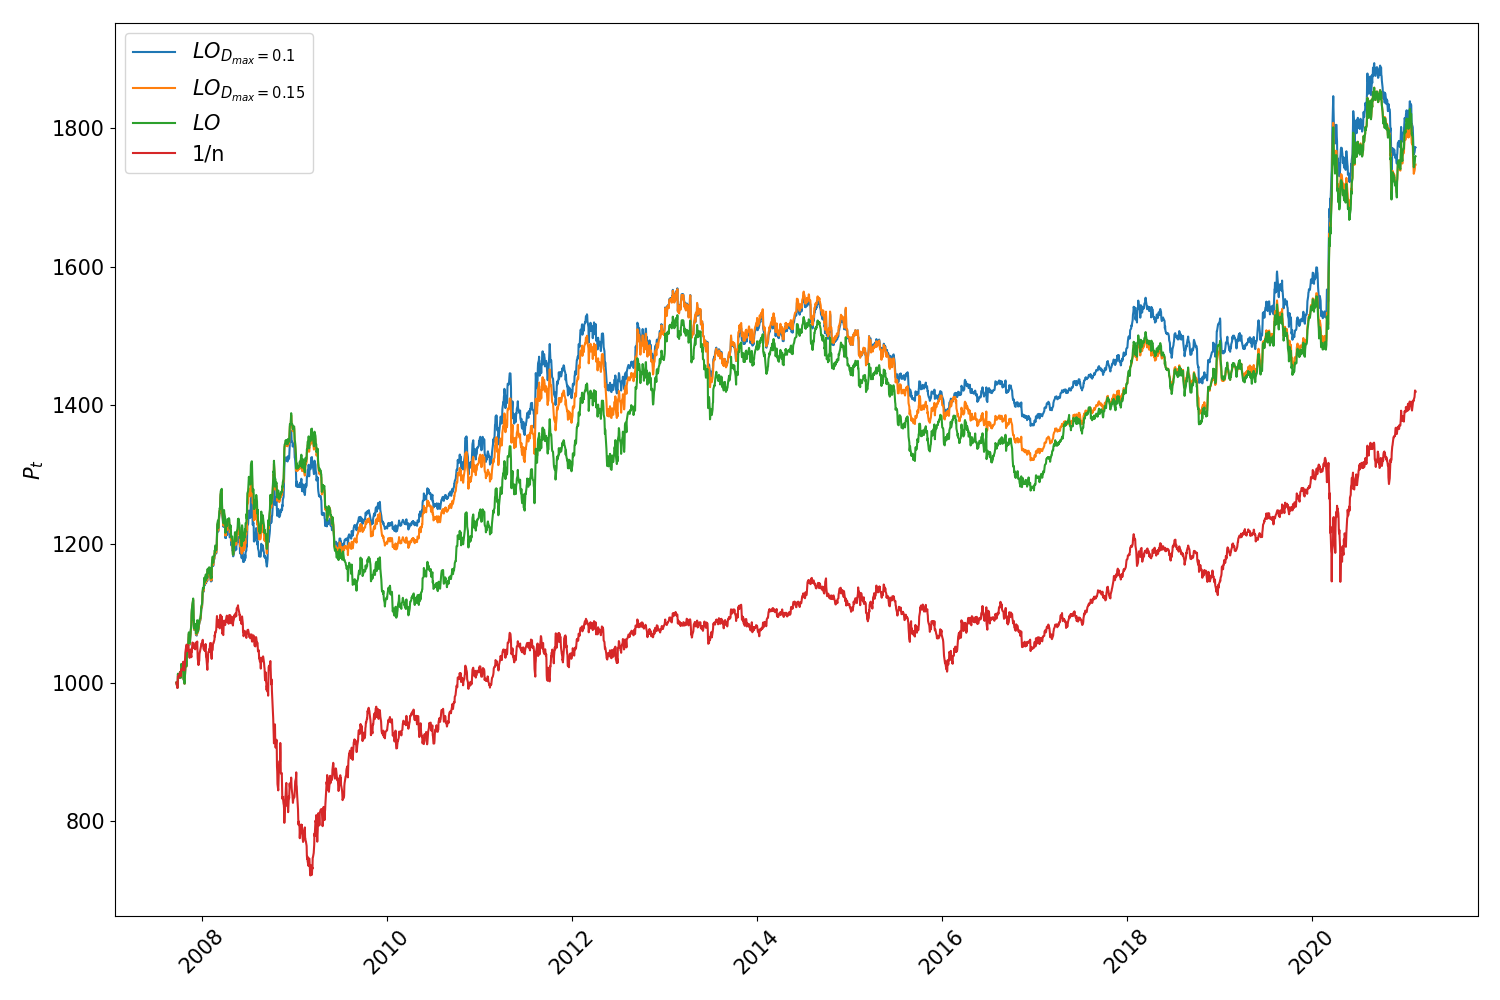
\includegraphics[width=1\textwidth]{analysis/portfolio_exercise/images/mle/port_vals_lo.png}
    \caption[Comparison of MPC investment strategies for various values of $D_{max}$]{Comparison of MPC investment strategies for various values of $D_{max}$.}
    \label{fig:MPC_port_vals_lo}
\end{figure}

\begin{figure}[H]
    \centering
    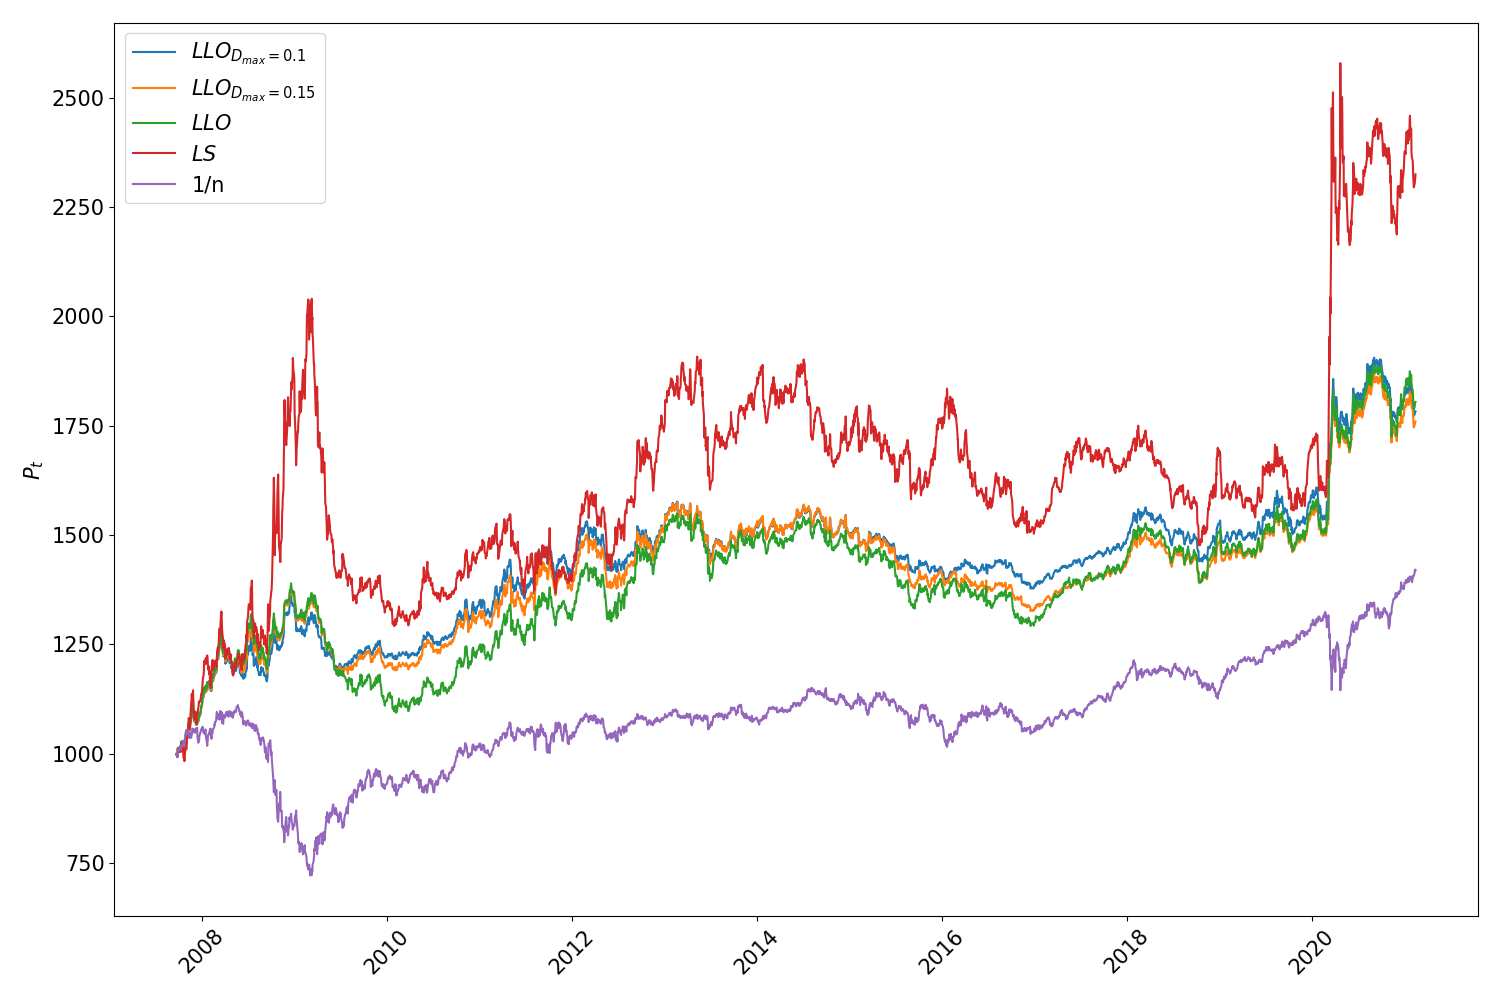
\includegraphics[width=1\textwidth]{analysis/portfolio_exercise/images/mle/port_vals_llo.png}
    \caption[Comparison of MPC investment strategies for various values of $D_{max}$]{Comparison of MPC investment strategies for various values of $D_{max}$.}
    \label{fig:MPC_port_vals_ls}
\end{figure}

\begin{figure}[H]
    \centering
    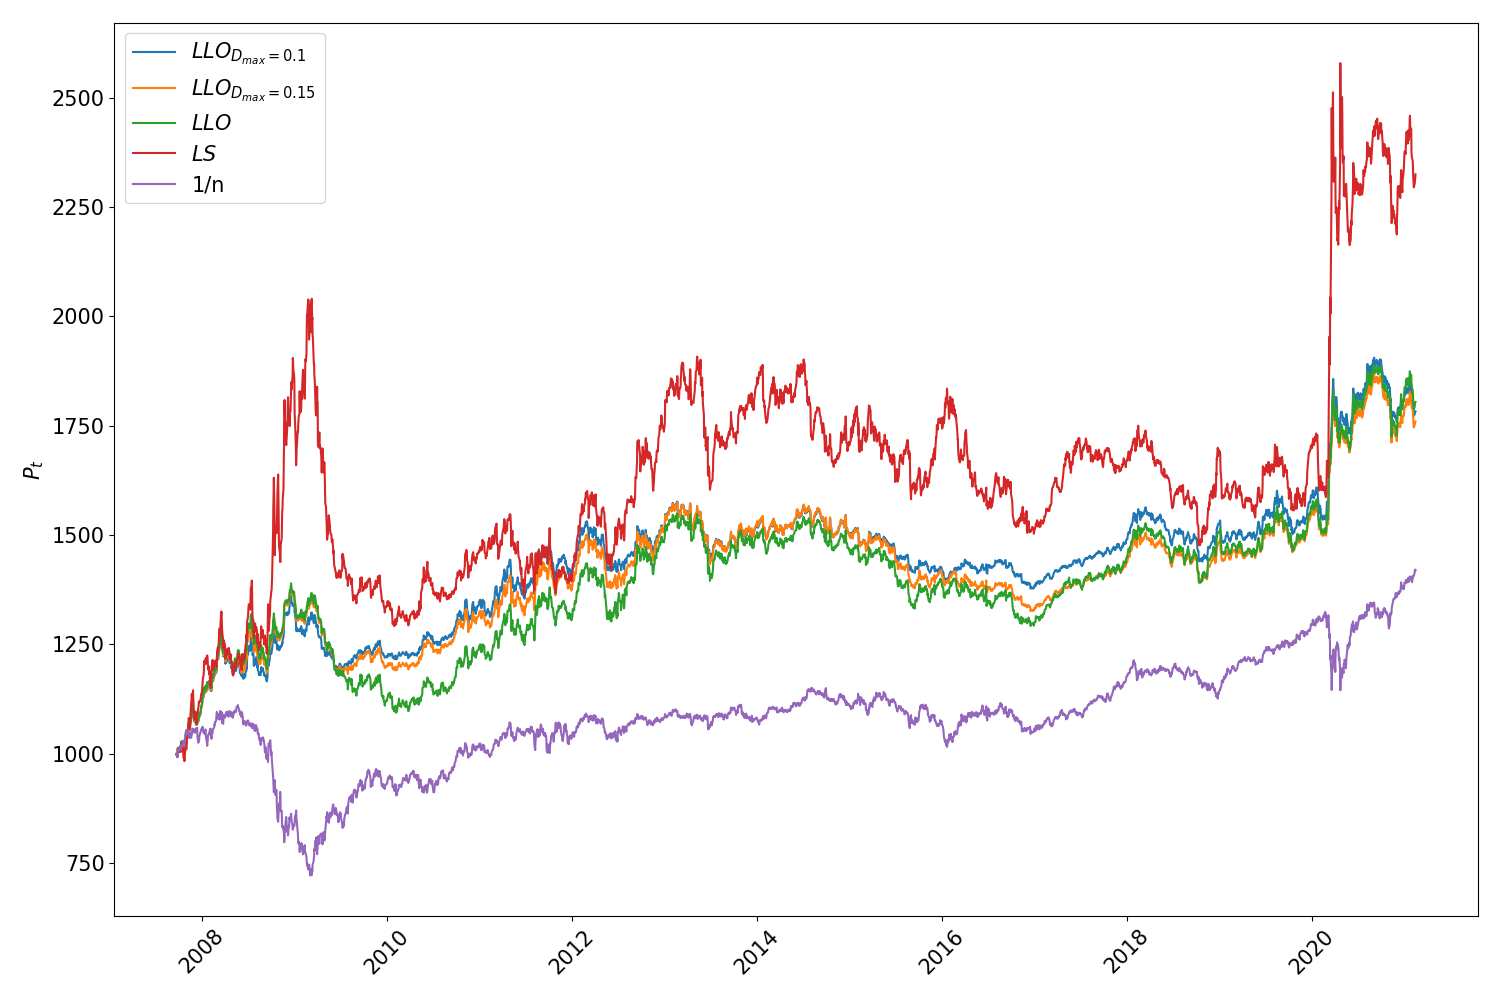
\includegraphics[width=1\textwidth]{analysis/portfolio_exercise/images/mle/port_vals_llo.png}
    \caption[Comparison of MPC investment strategies for various values of $D_{max}$]{Comparison of MPC investment strategies for various values of $D_{max}$.}
    \label{fig:MPC_port_vals_llo}
\end{figure}


\subsubsection*{Efficient frontiers long-only}

\textbf{Vi skal have udvalgt nogle enkelte plots herfra. Umiddelbart syntes jeg de plots med excess return på y-aksen skal fjernes. De plots med sharpe på y-aksen og henholdsvist $\gamma_0$, calmar ratio og maximum drawdown giver meget bedre mening --> Det er også de parametre vi optimerer imod in-sample.}

\begin{figure}[H]
    \centering
    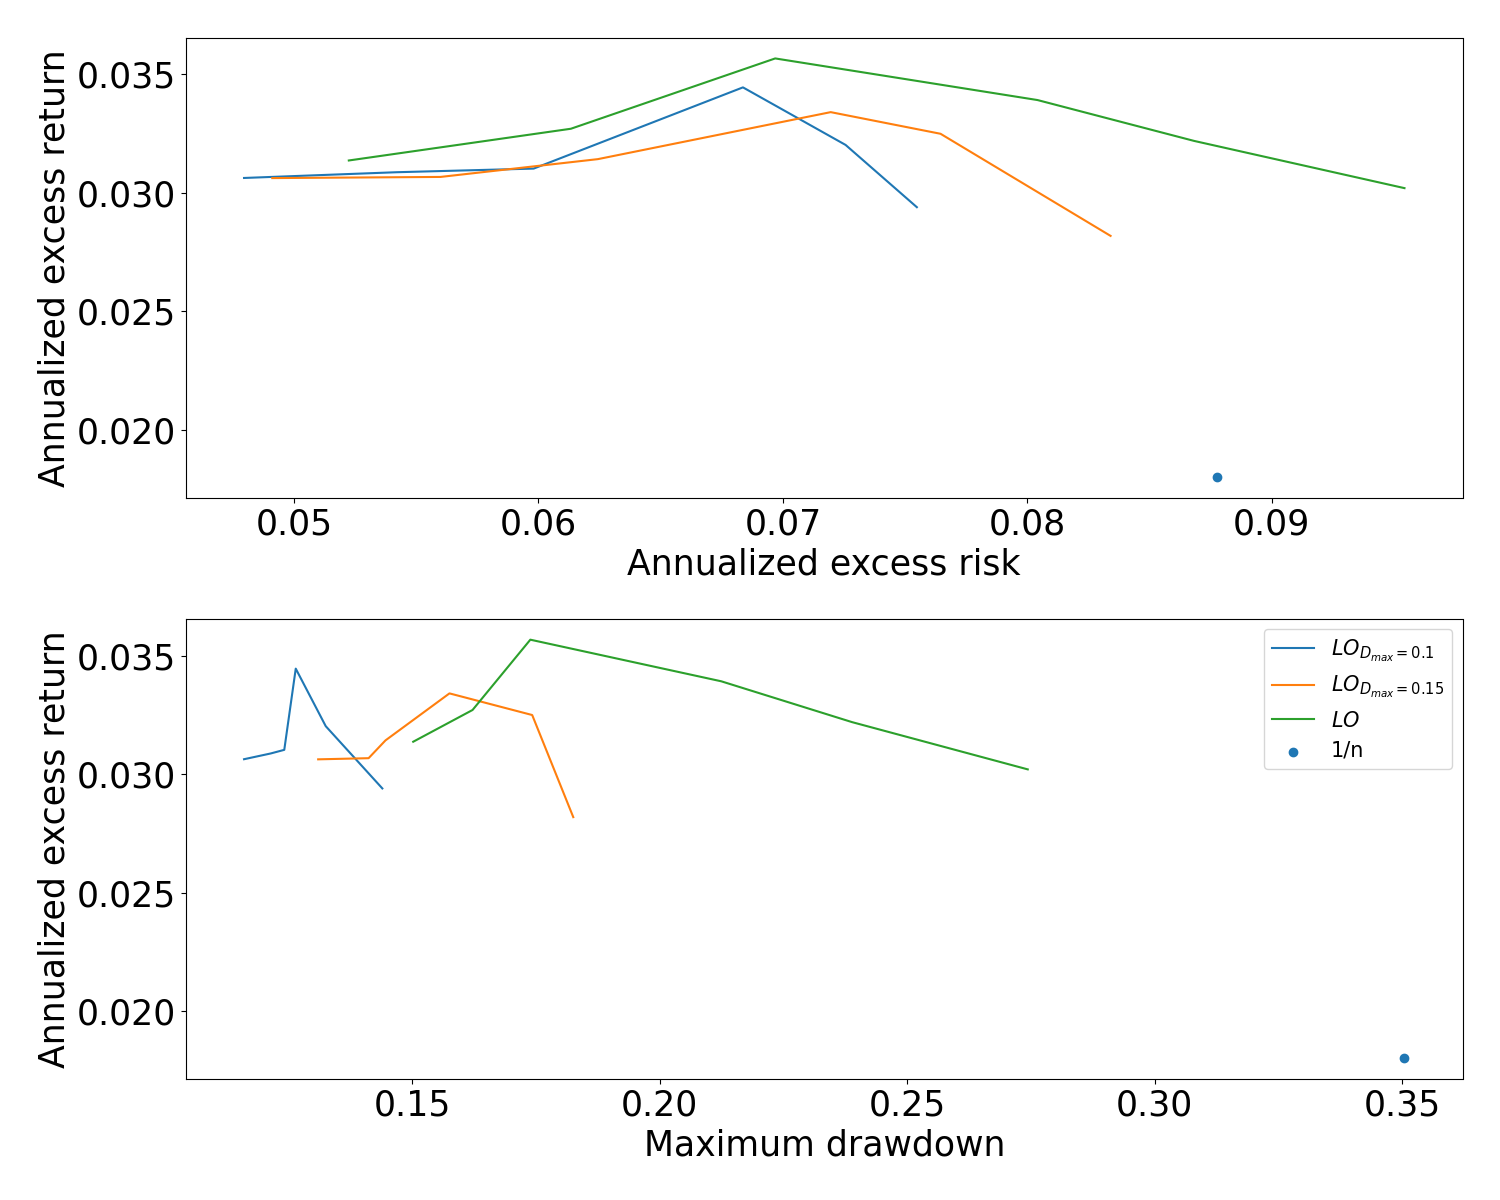
\includegraphics[width=1\textwidth]{analysis/portfolio_exercise/images/mle/frontier_lo.png}
    \caption[Efficient frontiers for various values of $D_{max}$]{Efficient frontiers for various values of $D_{max}$. The points from right to left correspond to $\gamma_0=1,3,5,10,15,25$}
    \label{fig:MPC_frontier_lo}
\end{figure}

\begin{figure}[H]
    \centering
    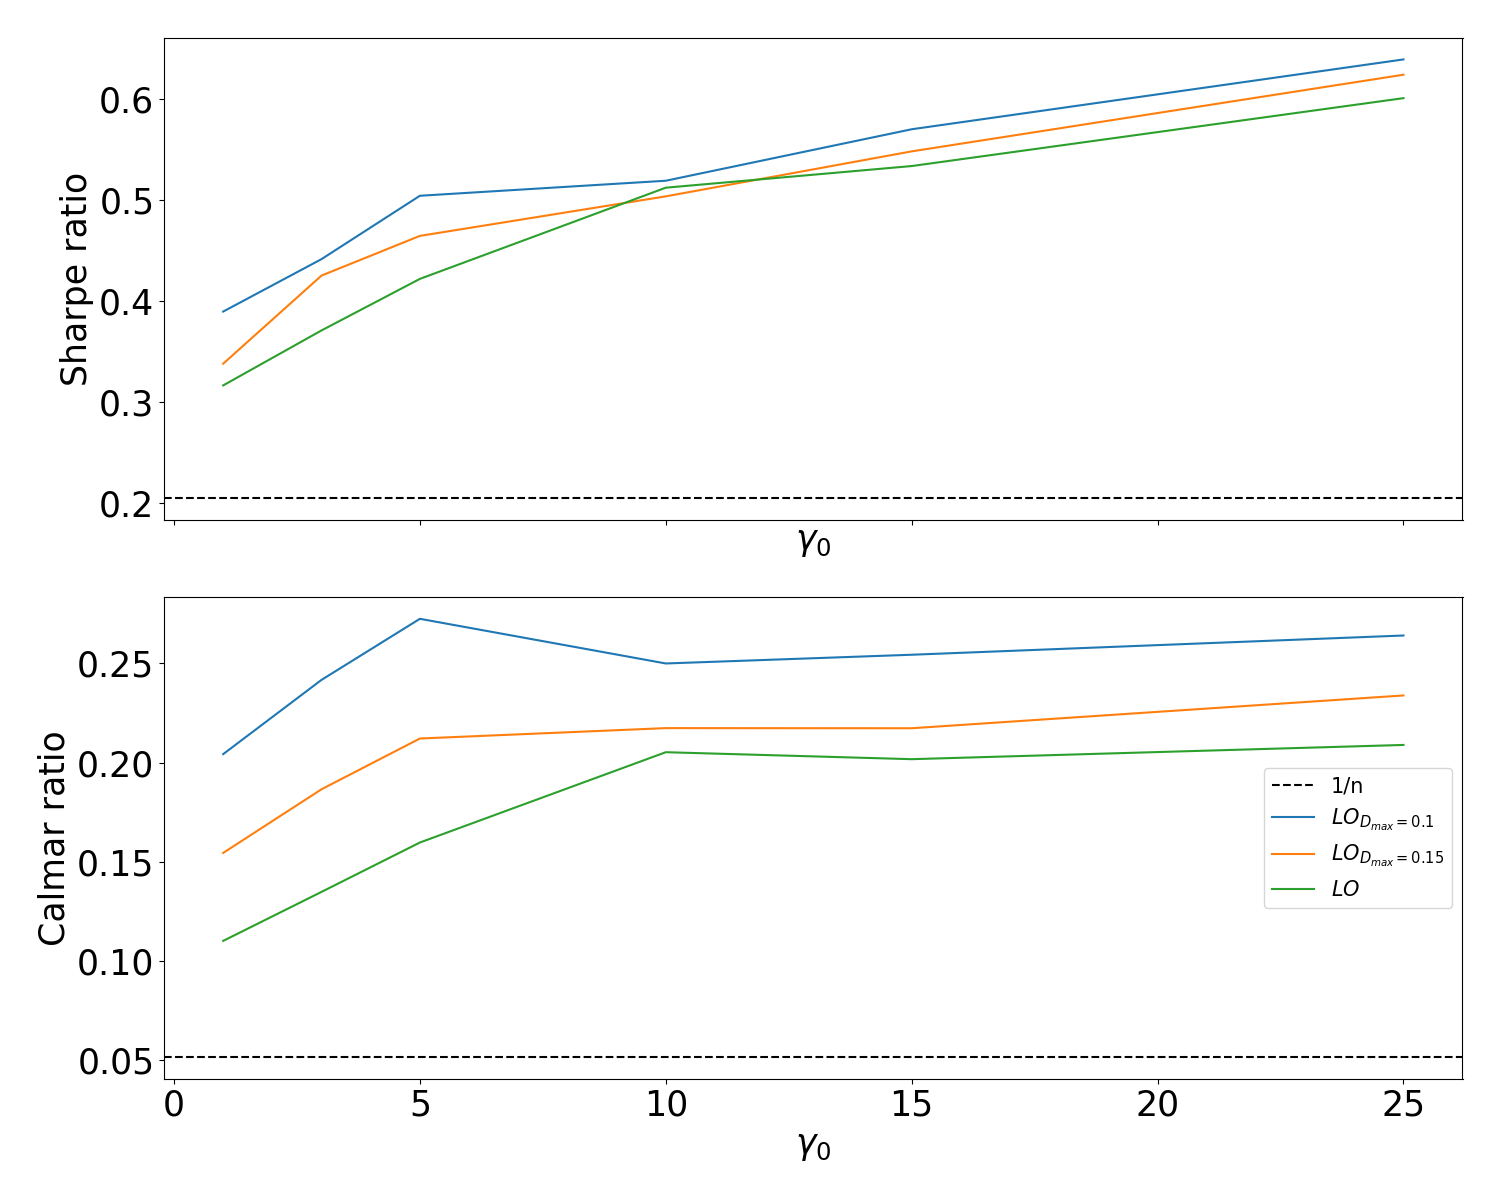
\includegraphics[width=1\textwidth]{analysis/portfolio_exercise/images/mle/sharpe_frontier_lo.png}
    \caption[Sharpe and Calmar ratio as function of $\gamma_0$ various values of $D_{max}$]{Sharpe and Calmar ratio as function of $\gamma_0$ various values of $D_{max}$.}
    \label{fig:MPC_sharpe_frontier_lo}
\end{figure}

\begin{figure}[H]
    \centering
    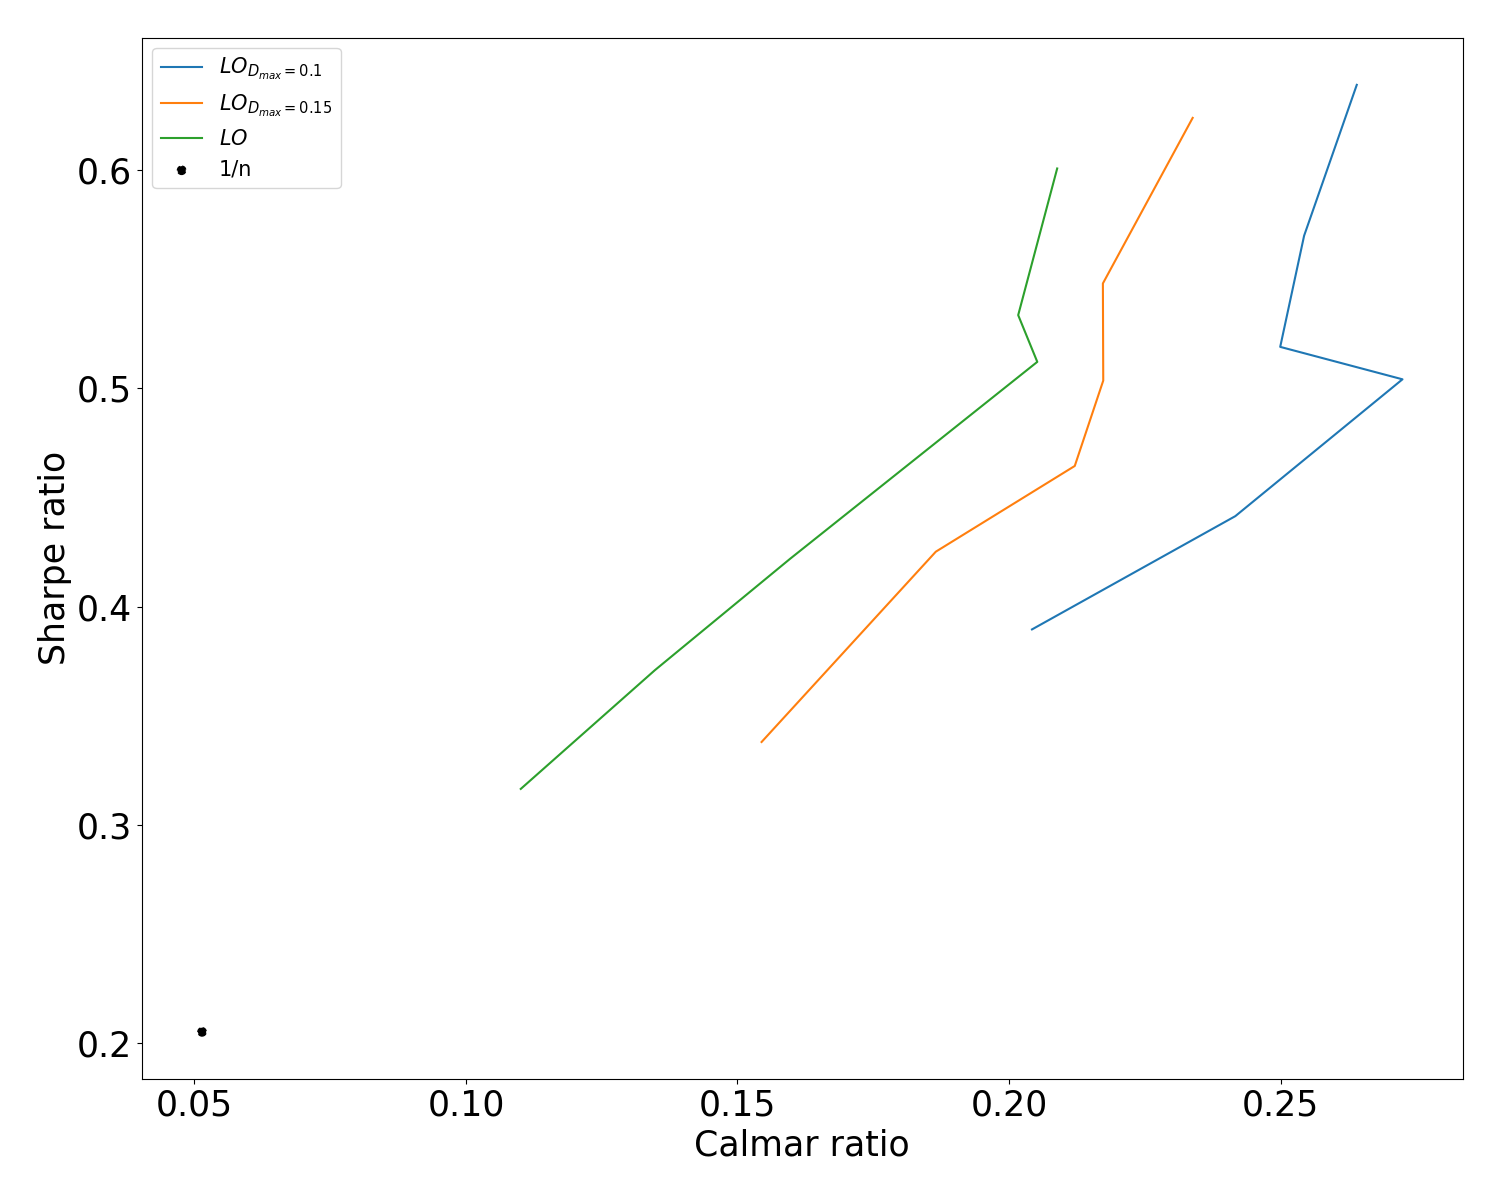
\includegraphics[width=1\textwidth]{analysis/portfolio_exercise/images/mle/sharpe_calmar_lo.png}
    \caption[Sharpe vs. Calmar ratio for various values of $D_{max}$]{Sharpe vs. Calmar ratio for various values of $D_{max}$. The points from left to right correspond to $\gamma_0=1,3,5,10,15,25$}
    \label{fig:MPC_sharpe_calmar_lo}
\end{figure}

\begin{figure}[H]
    \centering
    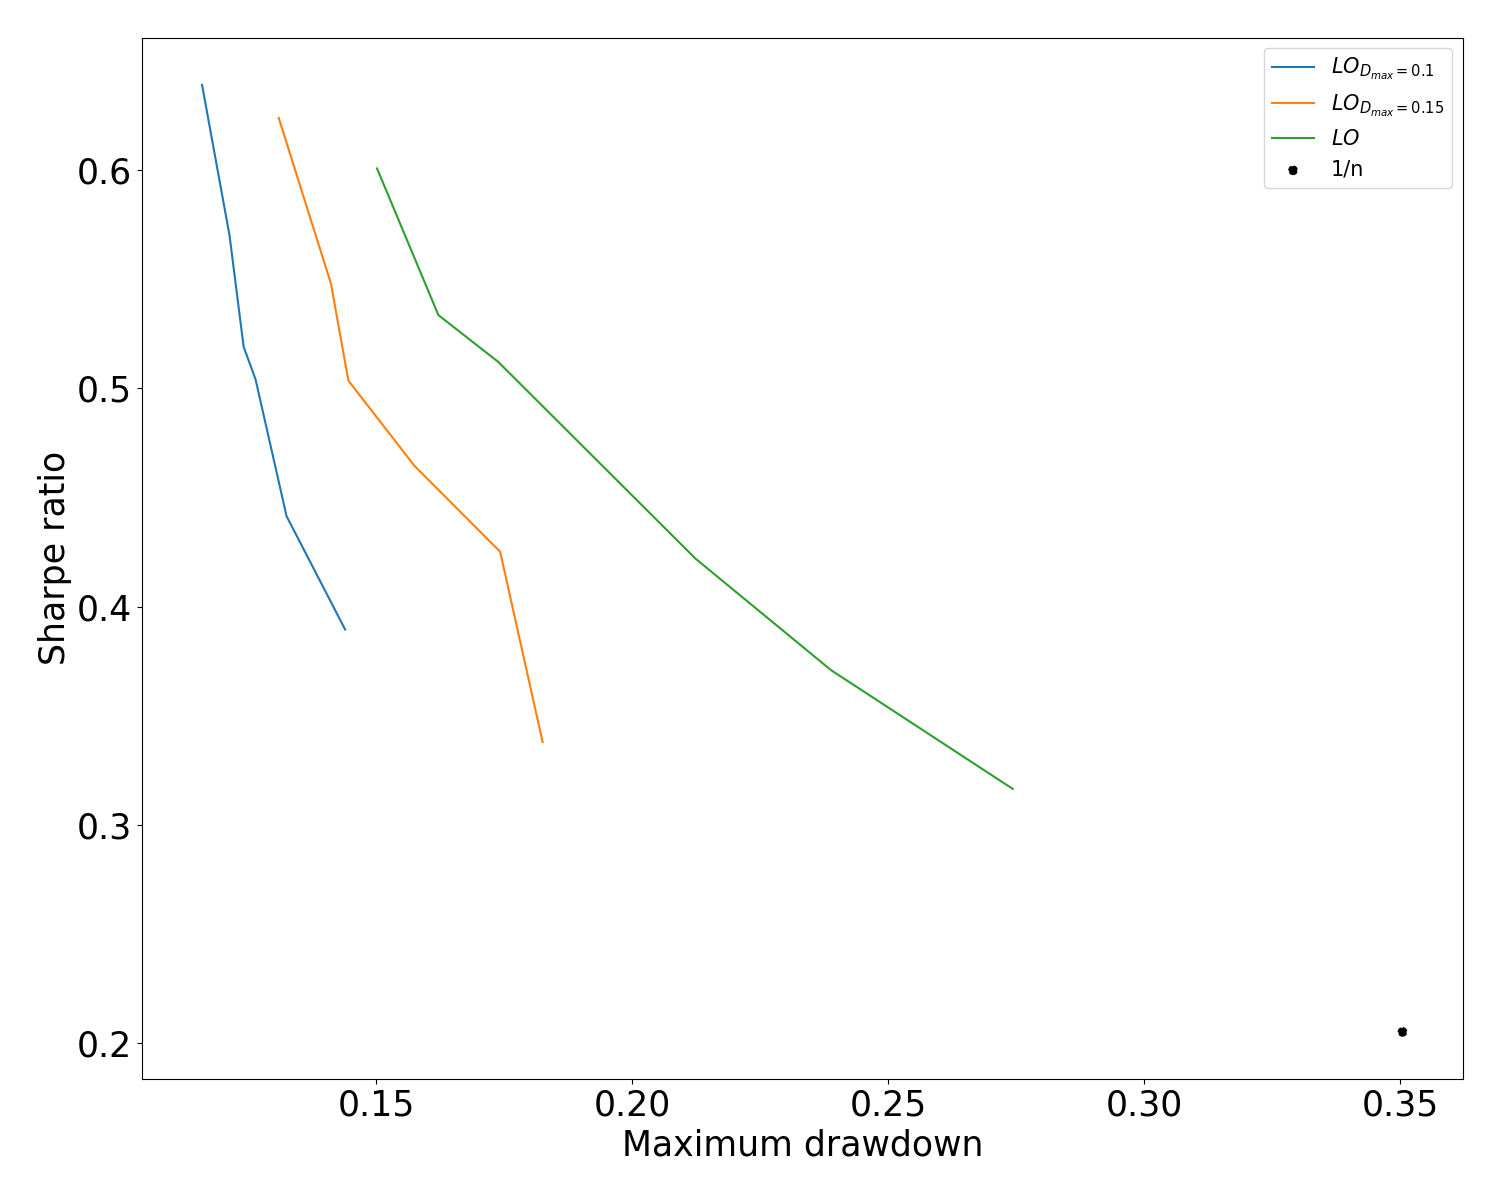
\includegraphics[width=1\textwidth]{analysis/portfolio_exercise/images/mle/sharpe_mdd_lo.png}
    \caption[Sharpe as function of MDD for various values of $D_{max}$]{Sharpe as function of MDD for various values of $D_{max}$. The points from right to left correspond to $\gamma_0=1,3,5,10,15,25$}
    \label{fig:MPC_sharpe_mdd_lo}
\end{figure}

\subsubsection*{Efficient frontiers long-short}

\begin{figure}[H]
    \centering
    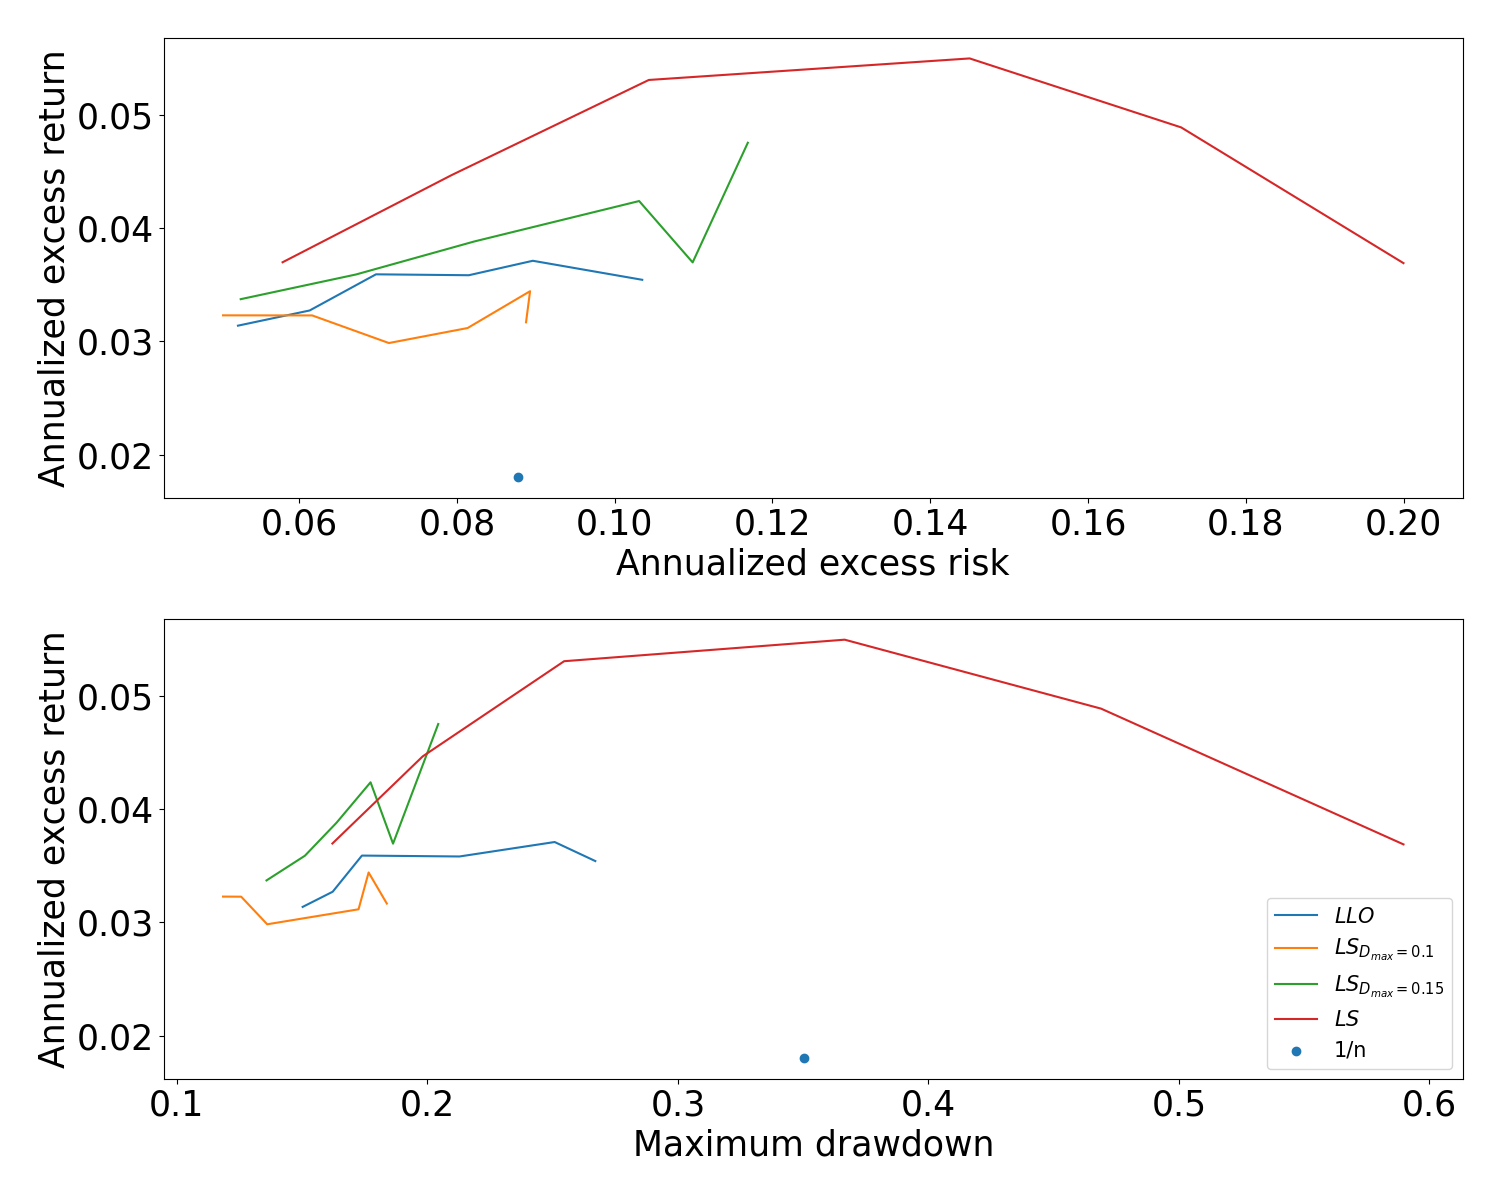
\includegraphics[width=1\textwidth]{analysis/portfolio_exercise/images/mle/frontier_ls.png}
    \caption[Efficient frontiers for various values of $D_{max}$]{Efficient frontiers for various values of $D_{max}$. The points from right to left correspond to $\gamma_0=1,3,5,10,15,25$}
    \label{fig:MPC_frontier_ls}
\end{figure}

\begin{figure}[H]
    \centering
    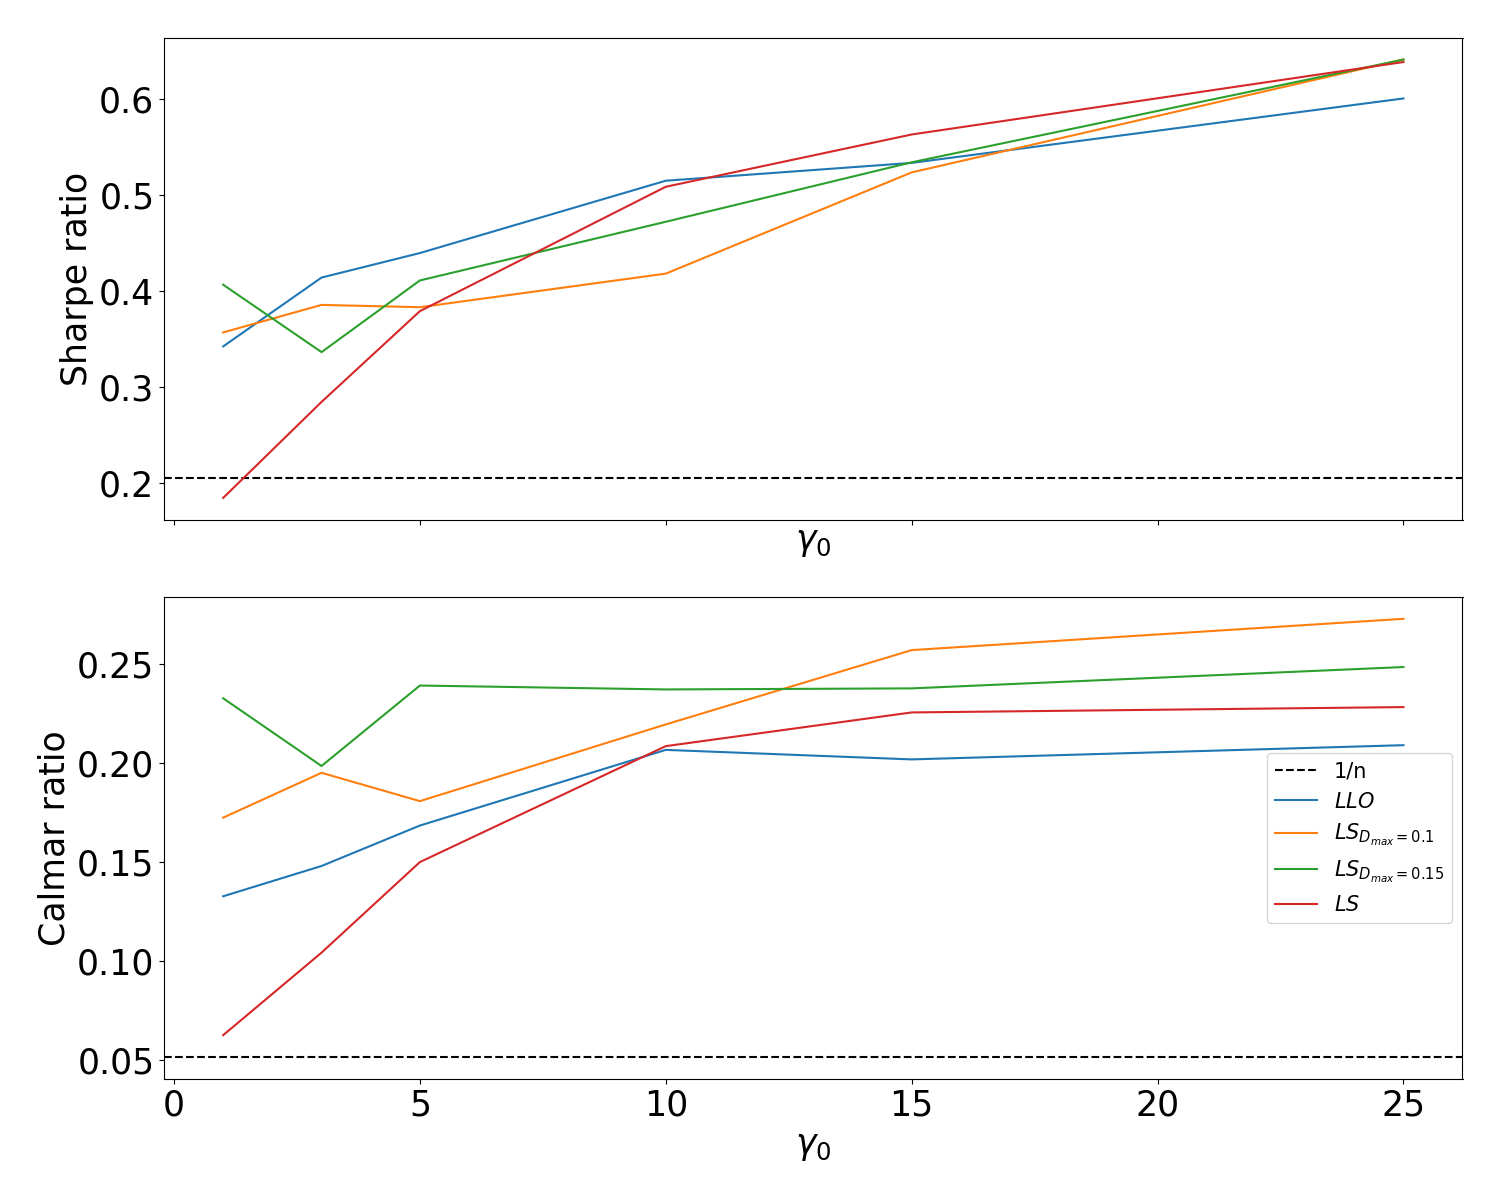
\includegraphics[width=1\textwidth]{analysis/portfolio_exercise/images/mle/sharpe_frontier_ls.png}
    \caption[Sharpe and Calmar ratio as function of $\gamma_0$ various values of $D_{max}$]{Sharpe and Calmar ratio as function of $\gamma_0$ various values of $D_{max}$.}
    \label{fig:MPC_sharpe_frontier_ls}
\end{figure}

\begin{figure}[H]
    \centering
    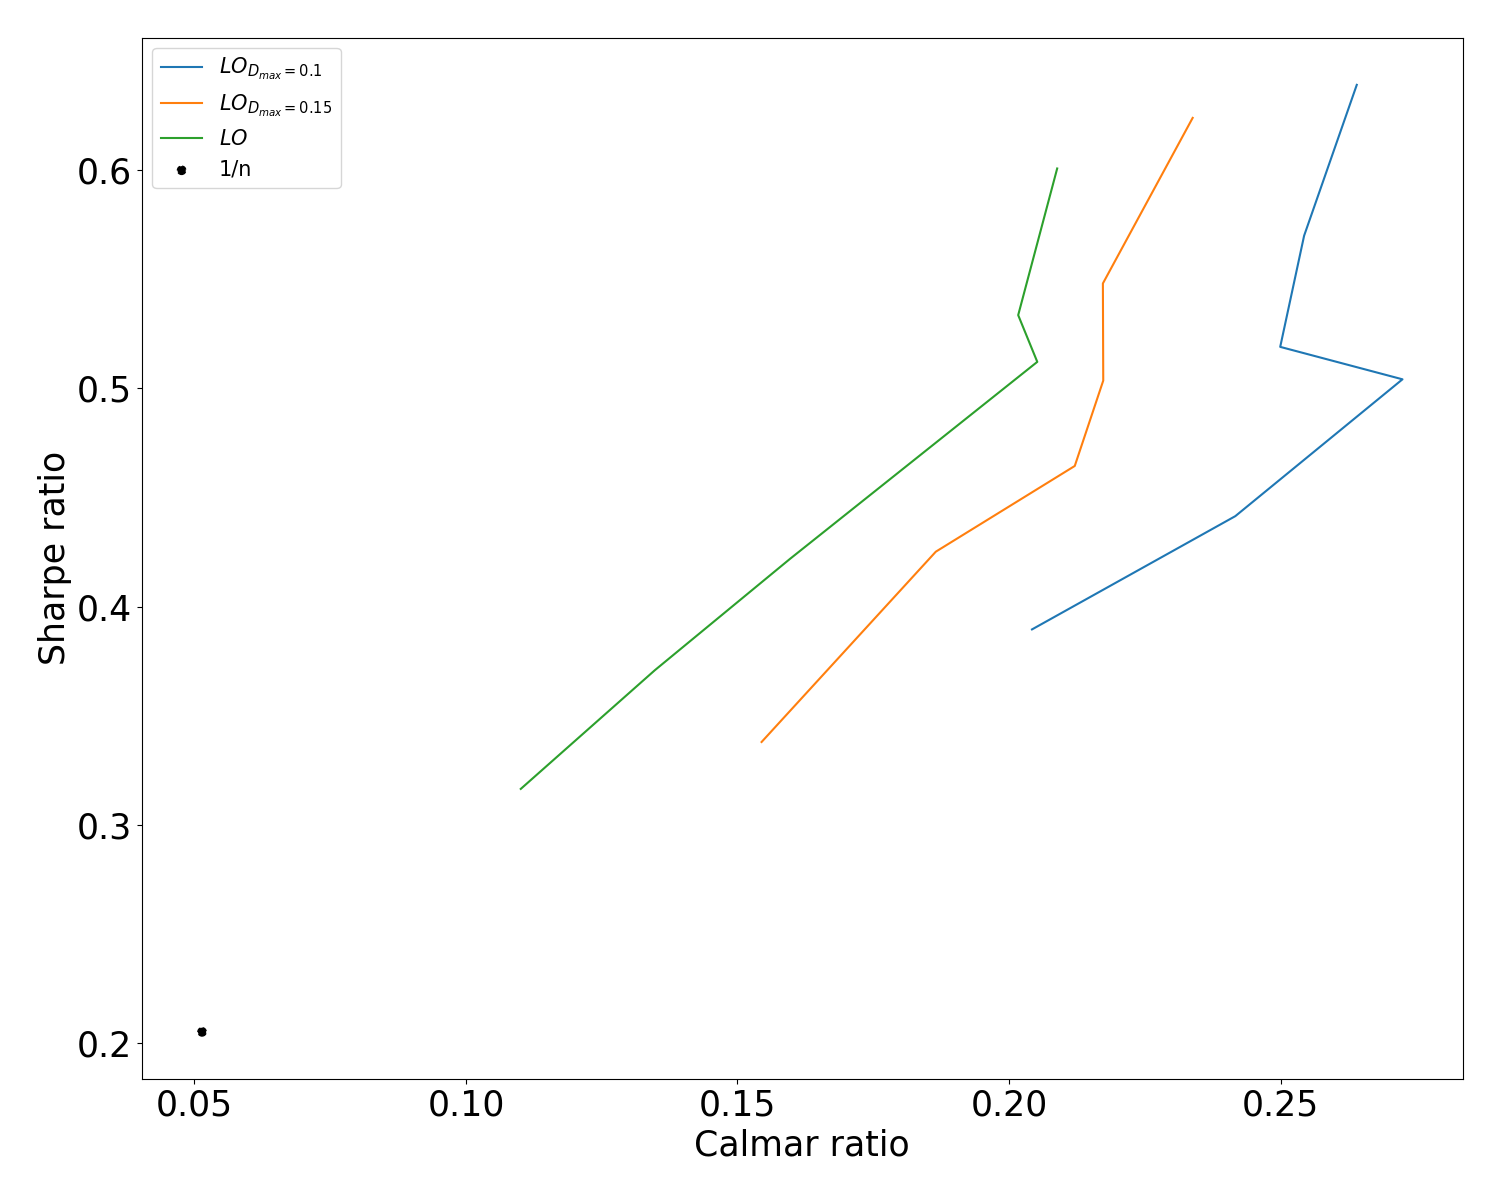
\includegraphics[width=1\textwidth]{analysis/portfolio_exercise/images/mle/sharpe_calmar_lo.png}
    \caption[Sharpe vs. Calmar ratio for various values of $D_{max}$]{Sharpe vs. Calmar ratio for various values of $D_{max}$. The points from left to right correspond to $\gamma_0=1,3,5,10,15,25$}
    \label{fig:MPC_sharpe_calmar_ls}
\end{figure}

\begin{figure}[H]
    \centering
    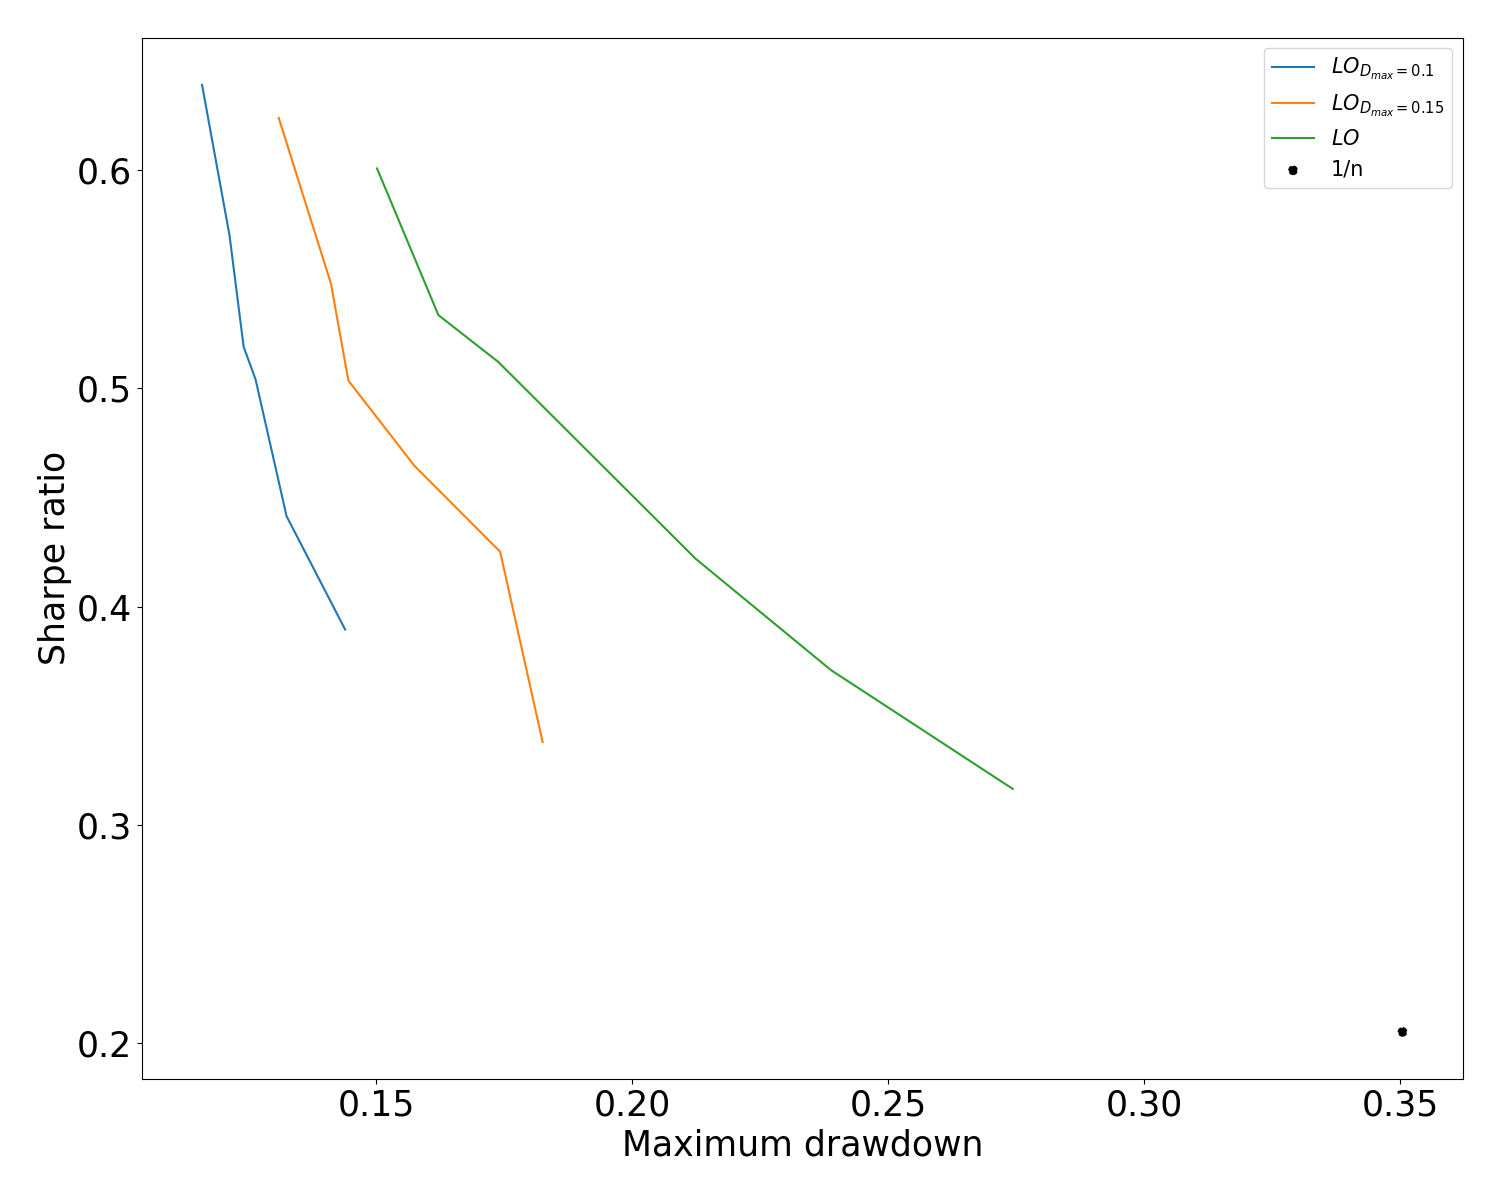
\includegraphics[width=1\textwidth]{analysis/portfolio_exercise/images/mle/sharpe_mdd_lo.png}
    \caption[Sharpe as function of MDD for various values of $D_{max}$]{Sharpe as function of MDD for various values of $D_{max}$. The points from right to left correspond to $\gamma_0=1,3,5,10,15,25$}
    \label{fig:MPC_sharpe_mdd_ls}
\end{figure}

\subsubsection*{Efficient frontiers leveraged long-only}

\begin{figure}[H]
    \centering
    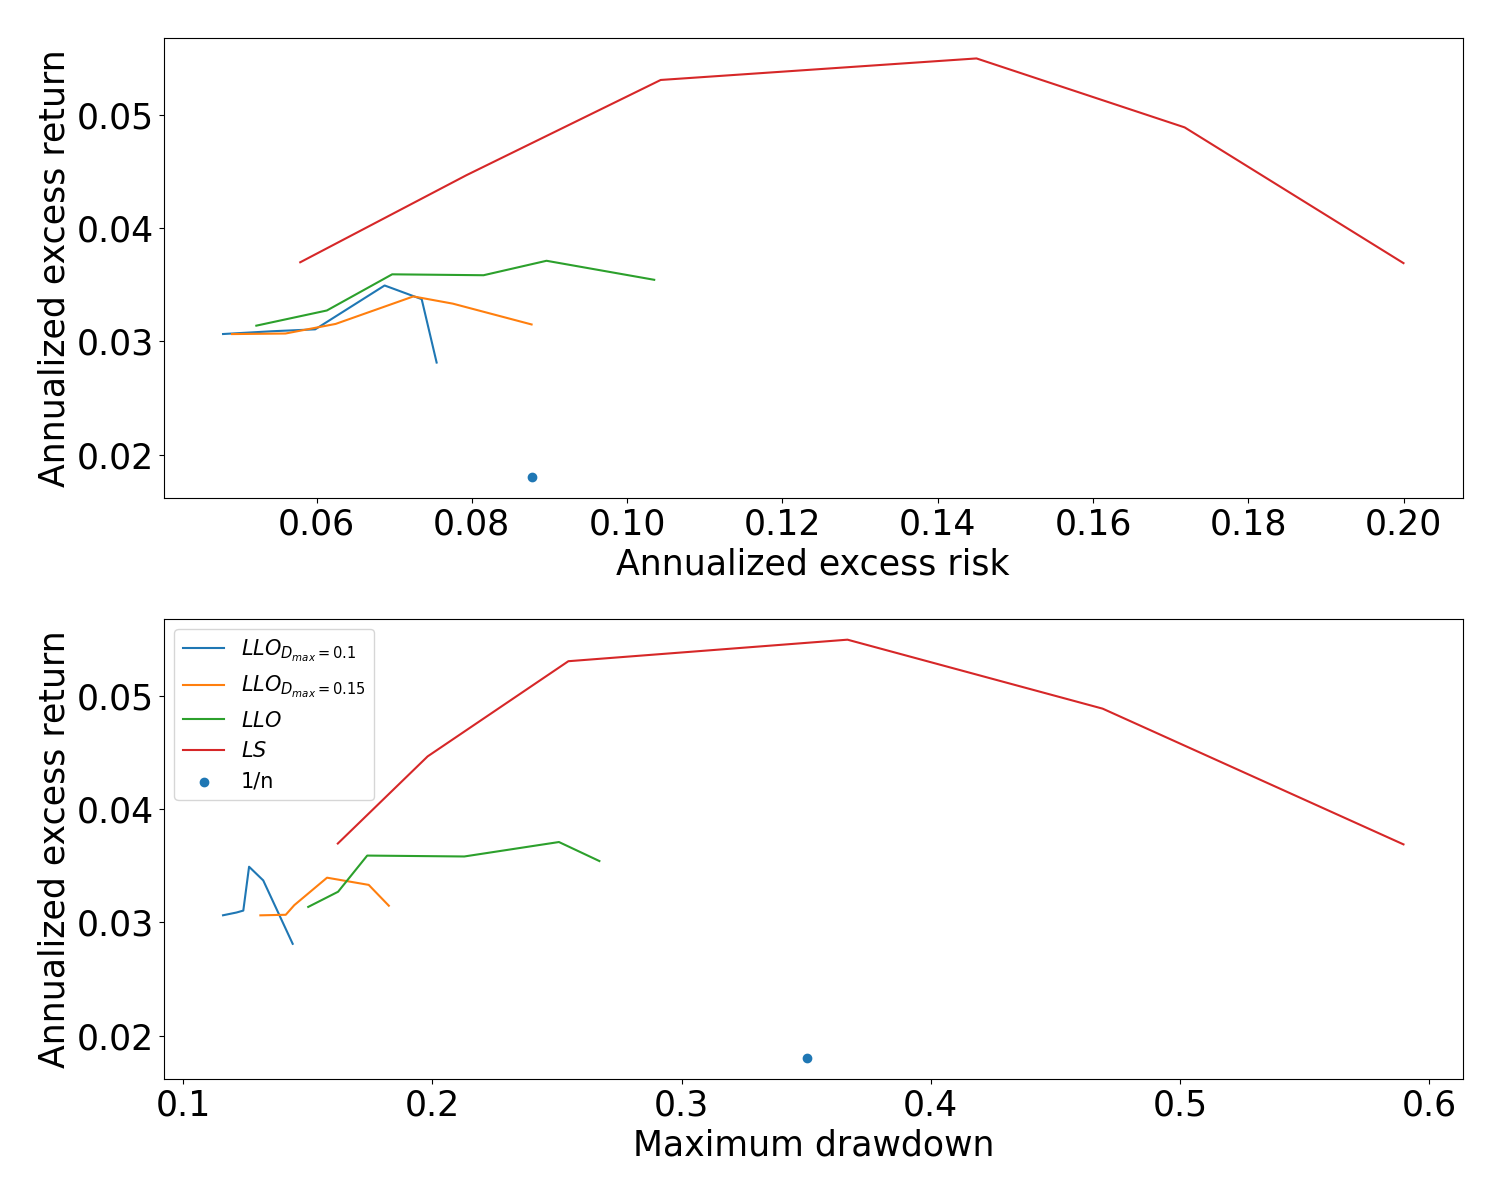
\includegraphics[width=1\textwidth]{analysis/portfolio_exercise/images/mle/frontier_llo.png}
    \caption[Efficient frontiers for various values of $D_{max}$]{Efficient frontiers for various values of $D_{max}$. The points from right to left correspond to $\gamma_0=1,3,5,10,15,25$}
    \label{fig:MPC_frontier_llo}
\end{figure}

\begin{figure}[H]
    \centering
    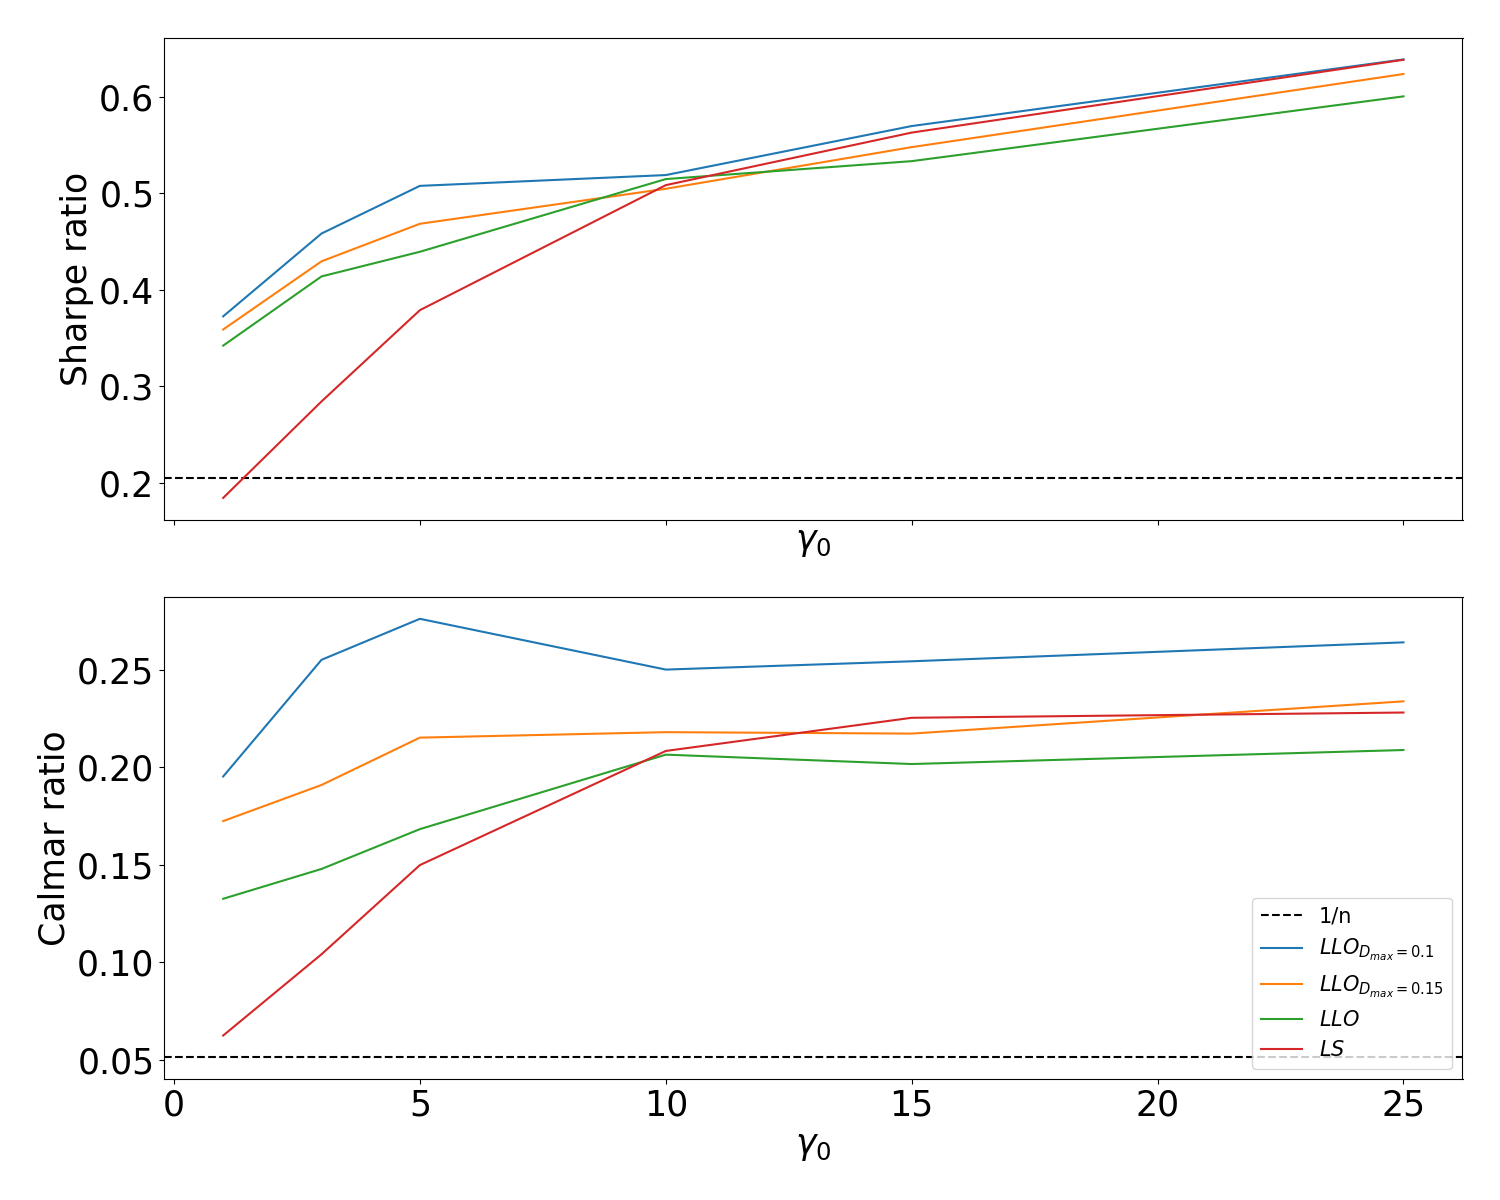
\includegraphics[width=1\textwidth]{analysis/portfolio_exercise/images/mle/sharpe_frontier_llo.png}
    \caption[Sharpe and Calmar ratio as function of $\gamma_0$ various values of $D_{max}$]{Sharpe and Calmar ratio as function of $\gamma_0$ various values of $D_{max}$.}
    \label{fig:MPC_sharpe_frontier_llo}
\end{figure}

\begin{figure}[H]
    \centering
    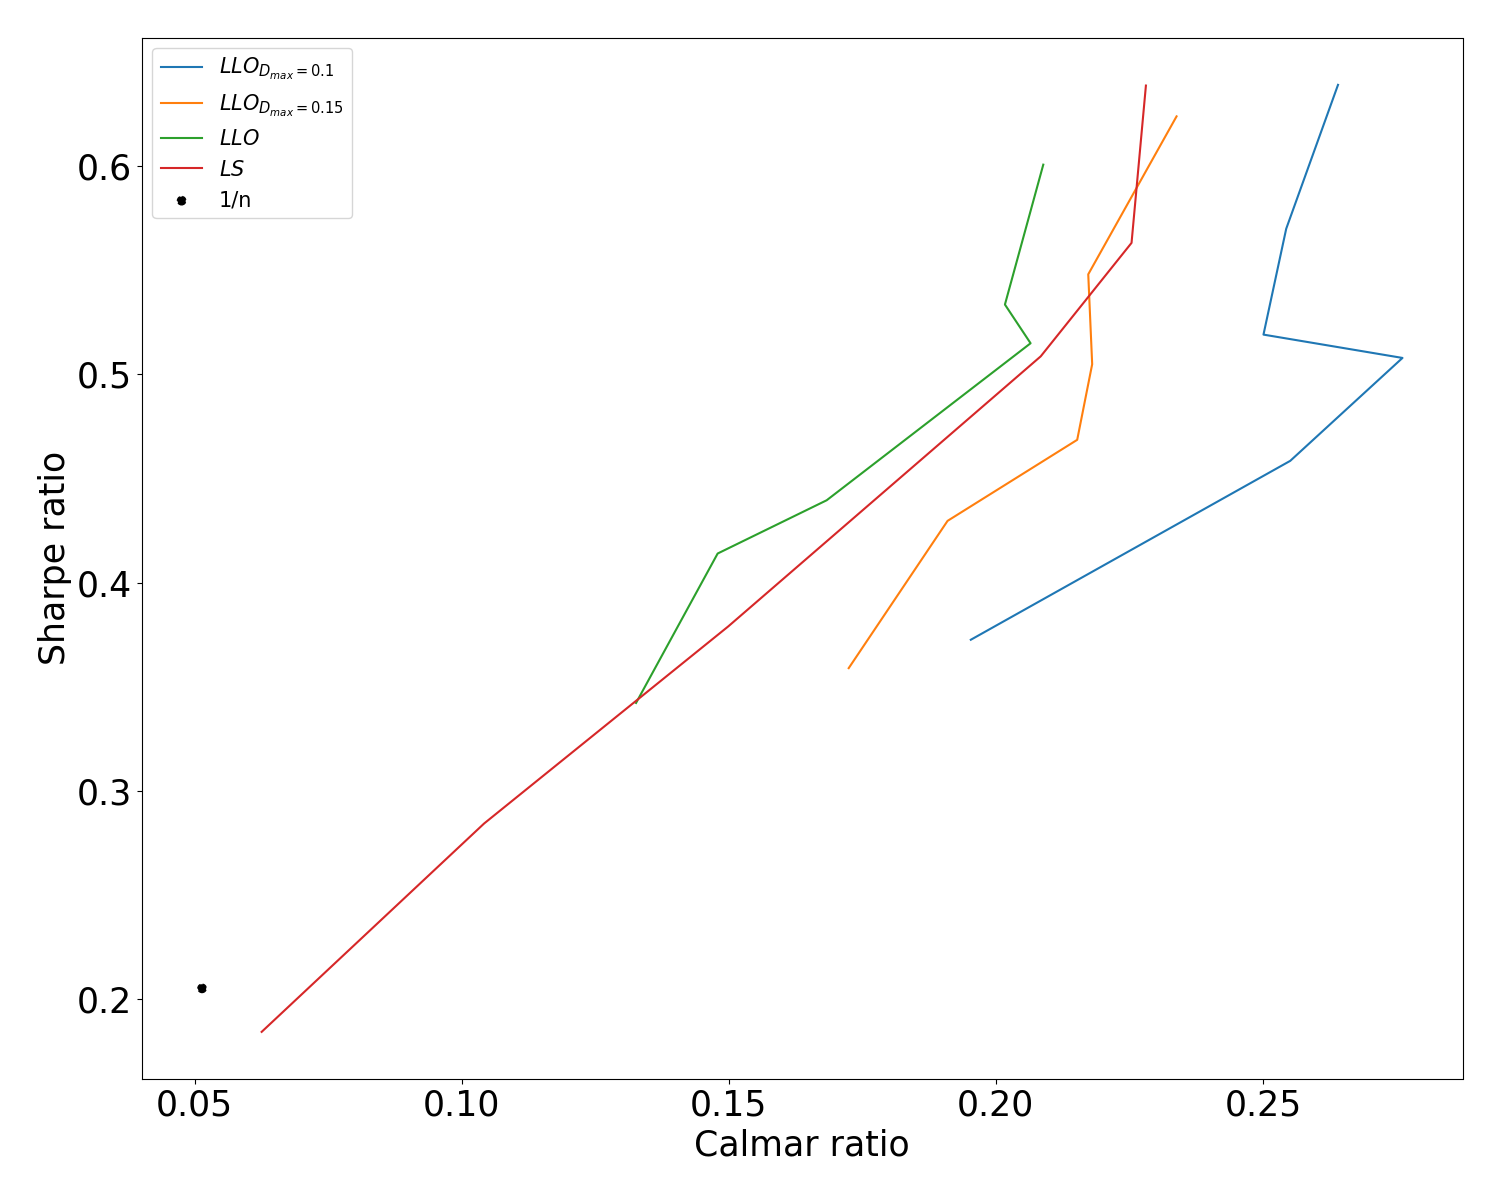
\includegraphics[width=1\textwidth]{analysis/portfolio_exercise/images/mle/sharpe_calmar_llo.png}
    \caption[Sharpe vs. Calmar ratio for various values of $D_{max}$]{Sharpe vs. Calmar ratio for various values of $D_{max}$. The points from left to right correspond to $\gamma_0=1,3,5,10,15,25$}
    \label{fig:MPC_sharpe_calmar_llo}
\end{figure}

\begin{figure}[H]
    \centering
    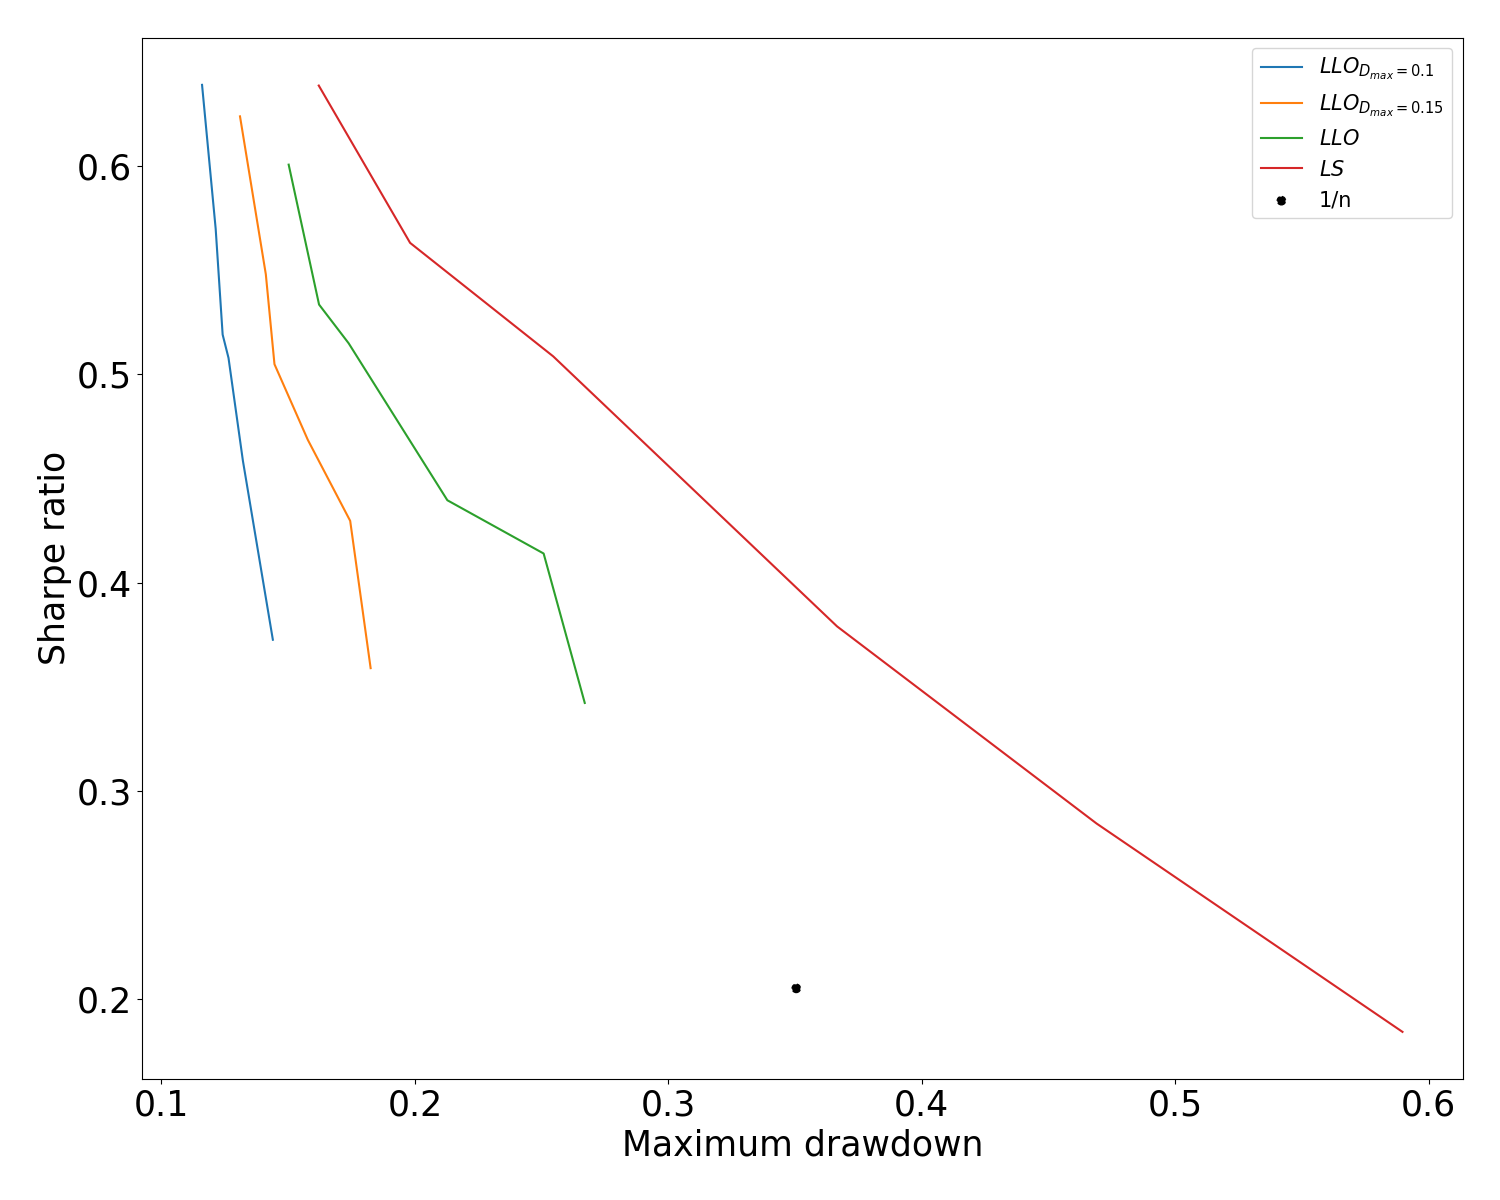
\includegraphics[width=1\textwidth]{analysis/portfolio_exercise/images/mle/sharpe_mdd_llo.png}
    \caption[Sharpe as function of MDD for various values of $D_{max}$]{Sharpe as function of MDD for various values of $D_{max}$. The points from right to left correspond to $\gamma_0=1,3,5,10,15,25$}
    \label{fig:MPC_sharpe_mdd_llo}
\end{figure}

\subsubsection{Comparison}



\subsubsection{Notes to self}


\textbf{Consider using rolling estimation of state sequence where only 1 new state is detected each time step(like in BP) - current approach estimates a new state sequence over entire rolling window at each timestep, which might make estimated means and covariances more unstable. Also, do we include rf in theestimates of mu and covariance matrix or how do we handle that asset?}

\textbf{Consider adding estimation section for portfolio allocation as in BP - trained on the same in-sample data as the rest.}